% Template: http://www.acm.org/publications/proceedings-template
\documentclass[sigconf]{acmart}
\usepackage{booktabs} % For formal tables
\usepackage{minted}
\usepackage{graphicx}
\usepackage{arydshln}


% Copyright
%\setcopyright{none}
%\setcopyright{acmcopyright}
%\setcopyright{acmlicensed}
\setcopyright{rightsretained}
%\setcopyright{usgov}
%\setcopyright{usgovmixed}
%\setcopyright{cagov}
%\setcopyright{cagovmixed}


% DOI
\acmDOI{10.475/123_4}

% ISBN
\acmISBN{123-4567-24-567/08/06}

%Conference
\acmConference[WOODSTOCK'97]{ACM Woodstock conference}{July 1997}{El
  Paso, Texas USA} 
\acmYear{1997}
\copyrightyear{2016}

\acmPrice{15.00}


\begin{document}
\title{Cudele: Programmable Consistency and Fault Tolerance}

\author{Blind Author}
\orcid{1234-5678-9012}
\affiliation{%
  \institution{Institute for Clarity in Documentation}
  \streetaddress{P.O. Box 1212}
  \city{Dublin} 
  \state{Ohio} 
  \postcode{43017-6221}
}
\email{blindauthor@corporation.com}

\begin{abstract}

HPC developers debate abandoning POSIX because the synchronization and
serialization overheads of providing strong consistency and durability are too
costly -- and often uneccessary -- for their applications.  Unfortunately,
designing near-POSIX file systems excludes applications that rely on strong
consistency or durability, forcing developers to re-write their applications or
deploy them on a different system.  We present a file system and API that
allows clients to specify their consistency/durability requirements and assign
them to subtrees in the namespace, allowing administrators to optimize subtrees
within the same namespace for different workloads.  We draw conclusions about
the performance impact of unexplored consistency/durability metadata designs
and show that strong consistency can cause a 104\(\times\) slow down while merging
updates (7\(\times\) slow down) and maintaining durability (\(10\times\) slow
down) have more reasonable costs.

\end{abstract}




%
% The code below should be generated by the tool at
% http://dl.acm.org/ccs.cfm
% Please copy and paste the code instead of the example below. 
%
\begin{CCSXML}
<ccs2012>
 <concept>
  <concept_id>10010520.10010553.10010562</concept_id>
  <concept_desc>Computer systems organization~Embedded systems</concept_desc>
  <concept_significance>500</concept_significance>
 </concept>
 <concept>
  <concept_id>10010520.10010575.10010755</concept_id>
  <concept_desc>Computer systems organization~Redundancy</concept_desc>
  <concept_significance>300</concept_significance>
 </concept>
 <concept>
  <concept_id>10010520.10010553.10010554</concept_id>
  <concept_desc>Computer systems organization~Robotics</concept_desc>
  <concept_significance>100</concept_significance>
 </concept>
 <concept>
  <concept_id>10003033.10003083.10003095</concept_id>
  <concept_desc>Networks~Network reliability</concept_desc>
  <concept_significance>100</concept_significance>
 </concept>
</ccs2012>  
\end{CCSXML}

\ccsdesc[500]{Computer systems organization~Embedded systems}
\ccsdesc[300]{Computer systems organization~Redundancy}
\ccsdesc{Computer systems organization~Robotics}
\ccsdesc[100]{Networks~Network reliability}

% We no longer use \terms command
%\terms{Theory}

\keywords{ACM proceedings, \LaTeX, text tagging}

\maketitle

\section{Introduction}

% What is the problem?
File system metadata services in HPC have scalability problems. It has been
shown that HPC workloads are metadata resource intensive because administrative
tasks, like checkpointing~\cite{bent_plfs_2009} or scanning the file
system~\cite{zheng:pdsw2014-batchfs}, on large data sets leads to contention
for the same directories and inodes ({\it
e.g.}, path traversal). Applications perform better with dedicated metadata
servers~\cite{sevilla:sc15-mantle, ren:sc2014-indexfs} but provisioning a
metadata server for every client is unreasonable. This problem is exacerbated
by current trends in HPC, where architectures are transitioning from complex
storage stacks with burst buffer, file system, object store, and tape tiers to
more simplified stacks with just a burst buffer and object
store~\cite{bent:login16-hpc-trends}; this puts more pressure on data access
because more requests end up hitting the same layer and latencies cannot be 
hidden while data migrates across tiers.

\begin{figure}[tb]
\centering
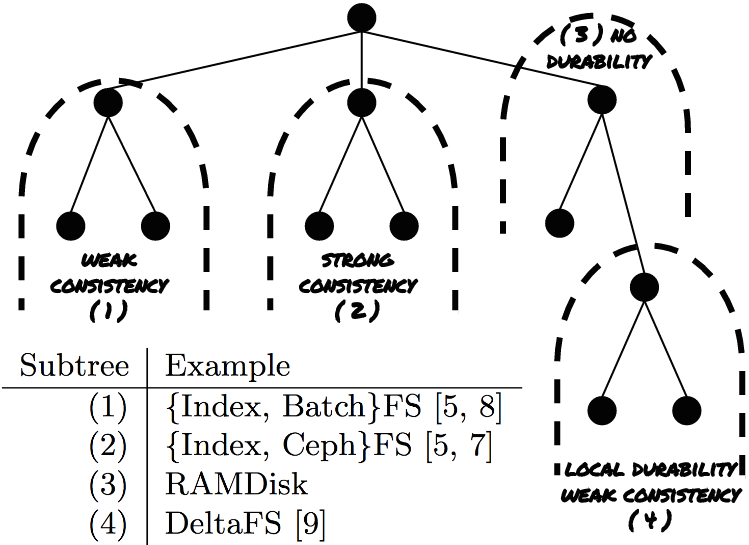
\includegraphics[width=0.5\textwidth]{figures/subtree-policies.png}
\caption{Administrators can assign consistency and durability policies to
subtrees to get the benefits of some of the state-of-the-art HPC architectures.
}\label{fig:subtree-policies}
\end{figure}


% What is HPC doing?
To address this, developers are relaxing the consistency and durability
semantics in the file system because weaker guarantees are sufficient for their
applications. For example, batch style jobs often do not need the strong
consistency that the file system provides, so
BatchFS~\cite{zheng:pdsw2014-batchfs} and DeltaFS~\cite{zheng:pdsw2015-deltafs}
do more client side processing and merge updates when the job is done. HPC
developers are turning to this non-POSIX solution because their applications
are well-understood ({\it e.g.}, well-defined read/write phases,
synchronization only needed during certain phases, workflows describing
computation, etc.) and because they wreak havoc on file systems designed for
general-purpose workloads ({\it e.g.}, checkpoint-restart's N-N and N-1 create
patterns).

% One example
One popular approach for relaxing consistency and durability is to ``decouple
the namespace", where clients lock the subtree they want exclusive access to as
a way to tell the file system that the subtree is important or may cause
resource contention in the near-future~\cite{grider:pdsw2015-marfs,
zheng:pdsw2015-deltafs, zheng:pdsw2014-batchfs, ren:sc2014-indexfs,
bent:slides-twotiers}. Then the file system can change its internal structure
to optimize performance. For example, the file system could enter a mode that
prevents other clients from interferring with the decoupled directory.  This
delayed merge ({\it i.e.} a form of eventual consistency) and relaxed
durability improves performance and scalability by avoiding the costs of RPCs,
synchronization, false sharing, and serialization.  The consistency and
durability semantics for these systems is shown in the table in
Figure~\ref{fig:subtree-policies} . While the performance benefits are obvious
for these users, applications that rely on the file system's guarantees must be
deployed on an entirely different system or re-written to coordinate strong
consistency/durability themselves.

%\begin{table}
%\begin{tabular}{ r | l }
%  Subtree         & Example \\\hline
%  (1)   & \{Index, Batch\}FS~\cite{ren:sc2014-indexfs, zheng:pdsw2014-batchfs} \\
%  (2)   & \{Index, Ceph\}FS~\cite{ren:sc2014-indexfs, weil:sc2004-dyn-metadata} \\
%  (3)   & RAMDisk \\
%  (4)   & DeltaFS~\cite{zheng:pdsw2015-deltafs} \\
%\end{tabular}
%
%\caption{State-of-the-art systems in HPC improve file system metadata
%performance by relaxing consistency and durability guarantees. Note that
%IndexFS also supports weak consistency with bulk inserts.
%\label{table:namespaces}} \end{table}

% What did we do
We propose subtree policies, an interface that lets future programmers control
the consistency and durability for subtrees in the file system namespace. For performance, one
subtree can adopt weaker consistency semantics while another subtree can retain
the rigidity of POSIX's strong consistency. Figure~\ref{fig:subtree-policies}
shows an example setup where a single global namespace has directories for
applications designed for different, state-of-the-art HPC architectures.  We
present Cudele, a prototype programmable file system that supports different
degrees of consistency and durability by exposing mechanisms used within the
file system as a client library.  Cudele supports 3 forms of consistency
(invisible, weak, and strong) and 3 degrees of durability (none, local, and
global) giving the administrator a wide range of policies and optimizations
that can be custom fit to an application. Our contributions: 

\begin{enumerate}

  \item a prototype that lets administrators program a range of
  consistency and durability semantics (9 permutations), allowing them to custom
  fit the storage system to the application.

  \item an API for programming consistency/durability policies and assigning
  them to subtrees in the file system namespace.

  \item a comparison of the strategies used in recently proposed research systems against
  previously unexplored metadata designs.

\end{enumerate}

% Results
Our results confirm the assertions of ``clean-state" research systems that
decouple namespaces; specifically that the technique drastically improve
performance (104\(\times\) speed up) but we go a step further by quantifying
the costs of merging updates (7\(\times\) slow down) and maintaining durability
(\(10\times\) slow down). We also show the effect of having a metadata specific
file format in systems that are based on in-memory data structures.
Section~\ref{sec:related-work} places Cudele in the context of other related
work. Section~\ref{sec:posix-overheads} quantifies the cost of POSIX
consistency and system-defined durability and
Section~\ref{sec:methodology-decoupled-namespaces} presents the Cudele
prototype and API. Section~\ref{sec:implementation} describes Cudele's
mechanisms and shows how re-using internal subsystems results in an
implementation of less than 500 lines of code. The evaluation in
Section~\ref{sec:evaluation} quantifies the overheads and performance gains of
explored and previously unexplored metadata designs.


%\section{Related Work} 
\label{sec:related-work}

% General
The bottlenecks associated with accessing POSIX file system metadata are not limited
to HPC workloads and the same challenges that plagued these systems for years are
finding their way into the cloud. Workloads that deal with many small files
({\it e.g.}, log processing and database
queries~\cite{thusoo:sigmod2010-facebook-infrastructure}) and large numbers of
simultaneous clients ({\it e.g.}, MapReduce
jobs~\cite{mckusick:acm2010-gfs-evolution}), are subject to the scalability of
the metadata service. The biggest challenge is that whenever a file
is touched the client must access the file's metadata and maintaining a file
system namespace imposes small, frequent accesses on the underlying storage
system~\cite{roselli:atec2000-FS-workloads}.  Unfortunately, scaling file
system metadata is a well-known problem and solutions for scaling data IO do
not work for metadata IO~\cite{roselli:atec2000-FS-workloads,
abad:techreport2012-fstrace, abad:ucc2012-mimesis,
alam:pdsw2011-metadata-scaling, weil:osdi2006-ceph}. There are two approaches
for improving the performance of metadata access.

\subsection{Metadata Load Balancing}

% approaches to load balancing (strong = more resuorces per unit work, weak =
% fixed resource per work unit)
One approach for improving metadata performance and scalability is to alleviate
overloaded servers by load balancing metadata IO across a cluster. Common
techniques include partitioning metadata when there are many writes and
replicating metadata when there are many reads. For example, IndexFS partitions
directories and clients write to different partitions by grabbing leases and
caching ancestor metadata for path traversal; it does well for strong scaling
because servers can keep more inodes in the cache which results in less RPCs.
Alternatively, ShardFS replicates directory state so servers do not need to
contact peers for path traversal; it does well for read workloads because all
file operations only require 1 RPC and for weak scaling because requests will
never incurr extra RPCs due to a full cache.  CephFS employs both techniques to
a lesser extent; directories can be replicated or sharded but the caching and
replication policies do not change depending on the balancing technique.
Despite the performance benefits these techniques add complexity and jeopardize
the robustness and performance characteristics of the metadata service because
the systems now need (1) policies to guide the migration decisions and (2)
mechanisms to address inconsistent states across servers.

% policies
Setting policies for migrations is arguably more difficult than adding the
migration mechanisms themselves.  For example, IndexFS and CephFS use the
GIGA+~\cite{patil:fast2011-giga} technique for partitioning directories at a predefined
threshold and using lazy synchronization to redirect queries to the server that
``owns" the targeted metadata.  Determining when to partition directories and
when to migrate the directory fragments are policies that vary between systems:
GIGA+ partitions directories when the size reaches a certain number of files
and migrates directory fragments immediately; CephFS partitions directories
when they reach a threshold size or when the write temperature reaches a
certain value and migrates directory fragments when the hosting server has more
load than the other servers in the metadata cluster. Another policy is when and
how to replicate directory state; ShardFS replicates immediately and
pessimistically while CephFS replicates only when the read temperature reaches
a threshold.  There is a wide range of policies and it is difficult to address
with tunables and hard-coded design decisions.

% addressing inconsistency
In addition to the policies, distributing metadata across a cluster requiress
distributed transactions and cache coherence protocols to ensure strong
consistency ({e.g.}, POSIX).  For example, ShardFS pessimistically replicates
directory state and uses optimistic concurrency control for conflicts; namely
it does the operation and if there is a conflict at verification time it falls
back to two-phase locking.  Another example is IndexFS's inode cache which
reduces RPCs by caching ancestor paths -- the locality of this cache can be
thrashed by random reads but performs well for metadata writes. For
consistency, writes to directories in IndexFS block until the lease expires
while writes to direcotries in ShardFS are slow for everyone as it either
requires serialization or locking with many servers; reads in IndexFS are
subject to cache locality while reads in ShardFS always resolve to 1 RPC.
Another example of the overheads of addressing inconsistency is how CephFS
maintains client sessions and inode caches for capabilities (which in turn make
metadata access faster). When metadata is exchanged between metadata servers
these sessions/caches must be flushed and new statistics exchanged with a
scatter-gather process; this halts updates on the directories and blocks until
the authoratitive metadata server responds.  These protocols are discusssed in
more detail in the next section but their inclusion here is a testament to the
complexity of migrating metadata.

%For metadata writes it does a distributed transaction; monotonic writes with
%concurrent clients fail and do pessimistic locking through a mediated lock
%server to ensure strong consistency, non-monotonic writes grab locks at every
%server. Zooming in on monotonic writes: if permissions increase it executes on
%a primary then non-primary, if permissions decrease it executes on all
%non-primary then on primary.

The conclusion we have drawn from this related work is that metadata protocols
have a bigger impact on performance and scalability than load balancing.  
Understanding these protocols helps load balancing and gives us a better
understanding of the metrics we should use to make migration decisions ({\it
e.g.}, which operations reflect the state of the system), what types of
requests cause the most load, and how an overloaded system reacts ({\it e.g.},
increasing latencies, lower throughput, etc.).

\subsection{Relaxing POSIX}

% POSIX 
POSIX workloads require strong consistency and many file systems improve
performance by reducing the number of remote calls per operation ({\it i.e.}
RPC amplification). As discussed in the previous section, caching with leases and
replication are popular approaches to reducing the overheads of path traversals
but their performance is subject to cache locality and the amount of available
resources, respectively; for random workloads larger than the cache extra RPCs
hurt performance~\cite{ren:sc2014-indexfs, weil:sc2004-dyn-metadata} and for write heavy workloads with more
resources the RPCs for invalidations are harmful. Another approach to reducing
RPCs is to use leases or capabilities.  


%IndexFS aggressively caches paths and
%handles permissions by handing out leases for metadata writes; metadata may
%only be modified when all leases have expired. 
%IndexFS~\cite{ren:sc2014-indexfs} aggressively caches pathnames and their
%permissions on the client servers. Modifications to metadata cached by clients
%is delayed until all client leases have expired. This reduces the RPC
%amplification to 1 when mutatating directory metadata ({\it e.g.,}
%\texttt{mkdir}, \texttt{chmod}, etc.) because clients are not querying metadata servers for
%path traversals. The disadvantage of this approach is the high latency of
%mutation operations (reads to filenames).  ShardFS~\cite{xiao:socc2015-shardfs}
%replicates metadata (specifically directory lookup state) across the metadata server
%cluster, reducing the RPC amplification to 1 for file operations ({e.g.,}
%\texttt{stat}, \texttt{chmod}, \texttt{chown}, etc.). Modifications to the
%directory lookup state are done with optimistic concurrecny control and fall
%back to retry if verification fails. The disadvantage of this appraoch is the
%high number of RPCs for maintaining directory metadata mutations (writes to
%directories).  CephFS also maintains an inode cache but its notion of leases
%are much shorter, on the order of microseconds.

% Non POSIX
High performance computing has unique requirements for file systems ({e.g.},
fast creates) and well-defined workloads (e.g., workflows) that make relaxing
POSIX sensible.  One popular approach is to allow clients to ``lock'' parts of
the namespace to improve performance and scalability by avoiding
synchronization, false sharing, and serialization.  BatchFS assumes the
application coordinates accesses to the namespace, so the clients can batch
local operations and merge with a global namespace image lazily. Similarily,
DeltaFS eliminates RPC traffic using subtree snapshots for non-conflicting
workloads and middleware for conflicting workloads. MarFS gives administrators
the ability to (1) lock ``project directories" and (2) allocate GPFS clusters
for demanding directory workloads. TwoTiers eliminates high-latencies by
storing metadata in a flash tier; apps lock the namespace so that metadata can
be accessed more quickly.  Unfortunately, decoupling the namespaces has costs:
(1) merging metadata state back into the global namespace is slow; (2) failures
are local to the failing node; and (3) the systems are not backwards
compatible. 

% NON POSIX
%Decoupling the namespaces has many advantages, including improved scalability,
%higher resource utilization, and better performance.  BatchFS and DeltaFS are
%near-POSIX filesystems that give clients the ability to decouple subtrees from
%the namespace so that the applications can execute metadata operations without
%synchronization and serialization.  These operations are applied to a local
%snapshot of the file system namespace and conflicts are resolved either by the
%application or by an external service . Applications link into a metadata
%server library to reduce resource utilization and code paths (e.g., no daemons
%and less interprocess communication). 

For (1), state-of-the-art systems manage consistency in non-traditional ways:
IndexFS maintains the global namespace but blocks operations from other clients
until the first client drops the lease, BatchFS does operations on a snapshot
of the namespace and merges batches of operations into the global namespace,
and DeltaFS never merges back into the global namespace. The merging for
BatchFS is done by an auxiliary metadata server running on the client and
conflicts are resolved by the application. Although DeltaFS never explicitly
merges, applications needing some degree of ground truth can either manage
consistency thesmelves on a read or add a bolt-on service to manage the
consistency.

For (2), if the client fails and stays down, all metadata operations on the
decoupled namespace are lost. If the client recovers, the on-disk structures
(for BatchFS and DeltaFS this is the SSTables used in TableFS) can be
recovered. In other words, the clients have state that cannot be recovered if
the node stays failed and any progress will be lost. This scenario is a
disaster for checkpoint-restart where missed cycles may cause the checkpoint to
bleed over into computation time.

For (3), decoupled namespace approaches sacrifice POSIX going as far as
requiring the application to link against the systems they want to talk to. In
today's world of software defined caching, this can be a problem for large data
centers with many types and tiers of storage. Despite well-known performance
problems POSIX and REST are the dominant APIs for data transfer.

Decoupling the namespace delays metadata consistency and sacrifices durability. 
As shown in Table~\ref{table:namespaces}, metadata consistency is
provided by capabilities and metadata durability is addressed with a journal.
\begin{table}
\begin{tabular}{ r | l | l }
              & Decoupled & Global    \\
              & Namespace & Namespace \\\hline
  Example     & BatchFS~\cite{zheng:pdsw2014-batchfs} & CephFS~\cite{weil:sc2004-dyn-metadata} \\
              & DeltaFS~\cite{zheng:pdsw2015-deltafs} & IndexFS~\cite{ren:sc2014-indexfs}      \\
  Consistency & eventual & strong     \\
  Durability  & node local & journal  \\
\end{tabular}
\caption{State-of-the-art systems in HPC improve file system metadata
performance by relaxing consistency and durability
guarantees.\label{table:namespaces}}
\end{table}



\section{POSIX Overheads}
\label{sec:posix-overheads}

\begin{figure}[tb]
\centering
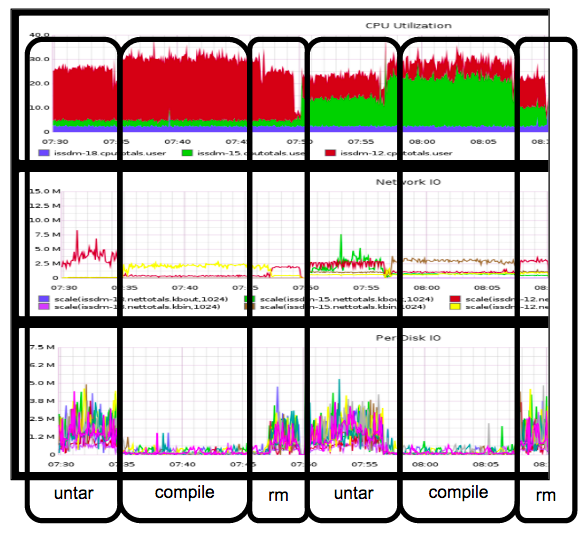
\includegraphics[width=1.0\linewidth]{figures/creates-motivation.png}
\caption{Create-heavy workloads (untar) incurr the highest disk, network, and
CPU utilization because of the consistency and durability demands of CephFS
.}\label{fig:creates-motivation}
\end{figure}

In our examiniation of the overheads of POSIX we benchmark and analyze CephFS,
the file system that uses the Ceph's object store ({\it i.e.} RADOS) to store
its data and metadata. We choose CephFS because it is an open-source production
quality system. This file system is an implementation of one set of design
decisions and our goal is to highlight the effect that those decisions have on
performance.

To show how the file system behaves under high metadata load we use a
create-heavy workload. Create-heavy workloads are studied the most in HPC
research because of the checkpoint/restart use case but they also happen to
stress the underyling storage system the most.
Figure~\ref{fig:creates-motivation} shows the resource utilization of compiling
the Linux kernel.  The untar phase, which is characterized by many creates, has
the highest resource usage which suggests that it is stressing the consistency
and journalling subsystems of the metadata server the most. Traditional file
system techniques for improving performance, such as caching inodes, do not
help for create-heavy workloads.

In this section, we quantify the costs of strong consistency and global
durability in CephFS.  We use the kernel client so that we can find the true
create speed of the server; our experiments show a low CPU utilziation for the
clients which indicates that we are stressing the servers more. 

\subsection{Durability}
\label{sec:fault-tolerance}

\begin{figure}[tb] \centering
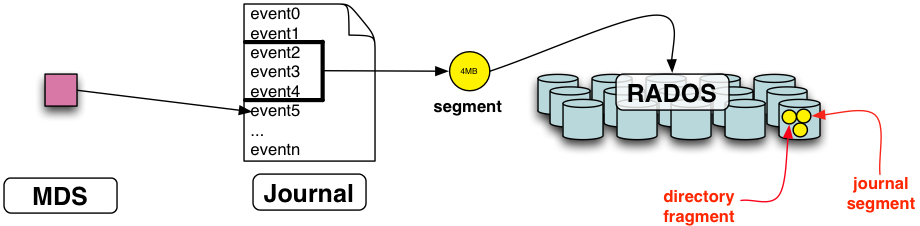
\includegraphics[width=1\linewidth]{./figures/journal.png} 
\caption{CephFS uses a journal to stage updates and tracks dirty metadata in
the collective memory of the MDSs. Each MDS maintains its own journal, which is
broken up into 4MB segments. These segments are pushed into RADOS and deleted
when that particular segment is trimmed from the end of the log. In addition to
journal segments, RADOS also stores per-directory objects. \label{fig:journal}}
\end{figure}
\begin{figure*}[t]
  \centering
  \begin{subfigure}[b]{.3\linewidth}
      \centering
      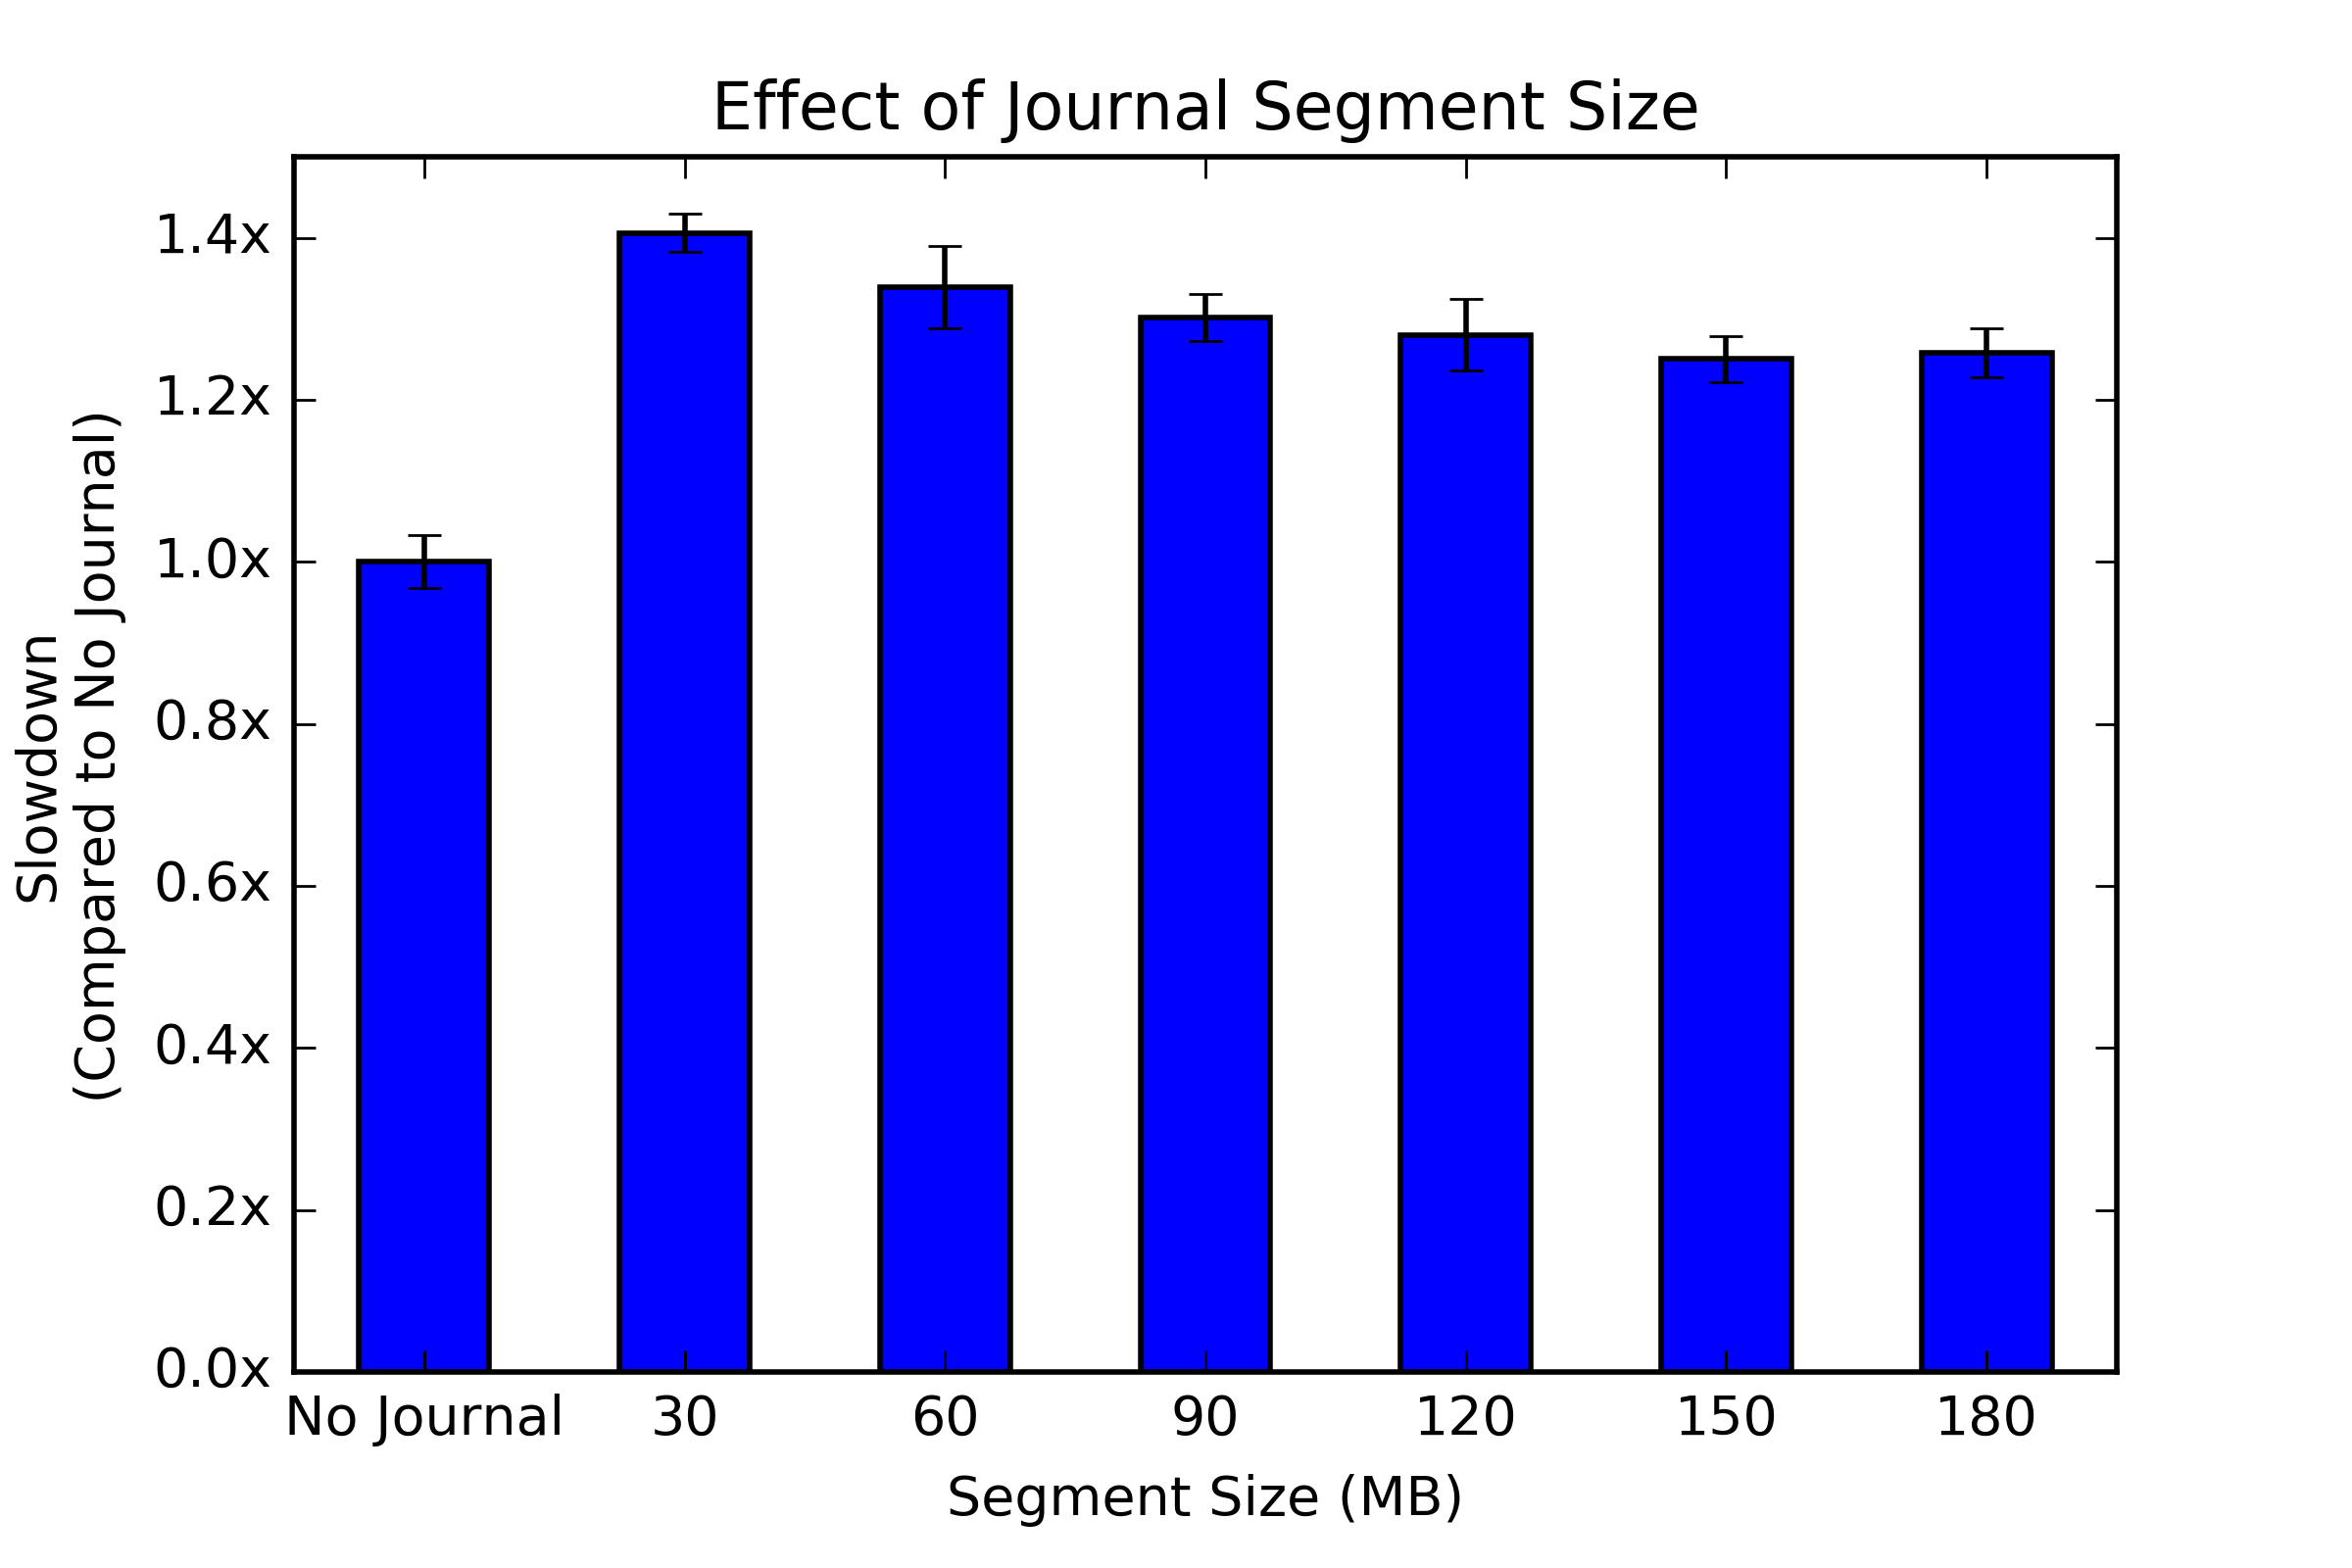
\includegraphics[width=1.0\linewidth]{graphs/slowdown-journal.png}
      \caption{Journal Segment Size} \label{fig:slowdown-journal-a}
  \end{subfigure}
  \begin{subfigure}[b]{.3\linewidth}
      \centering
      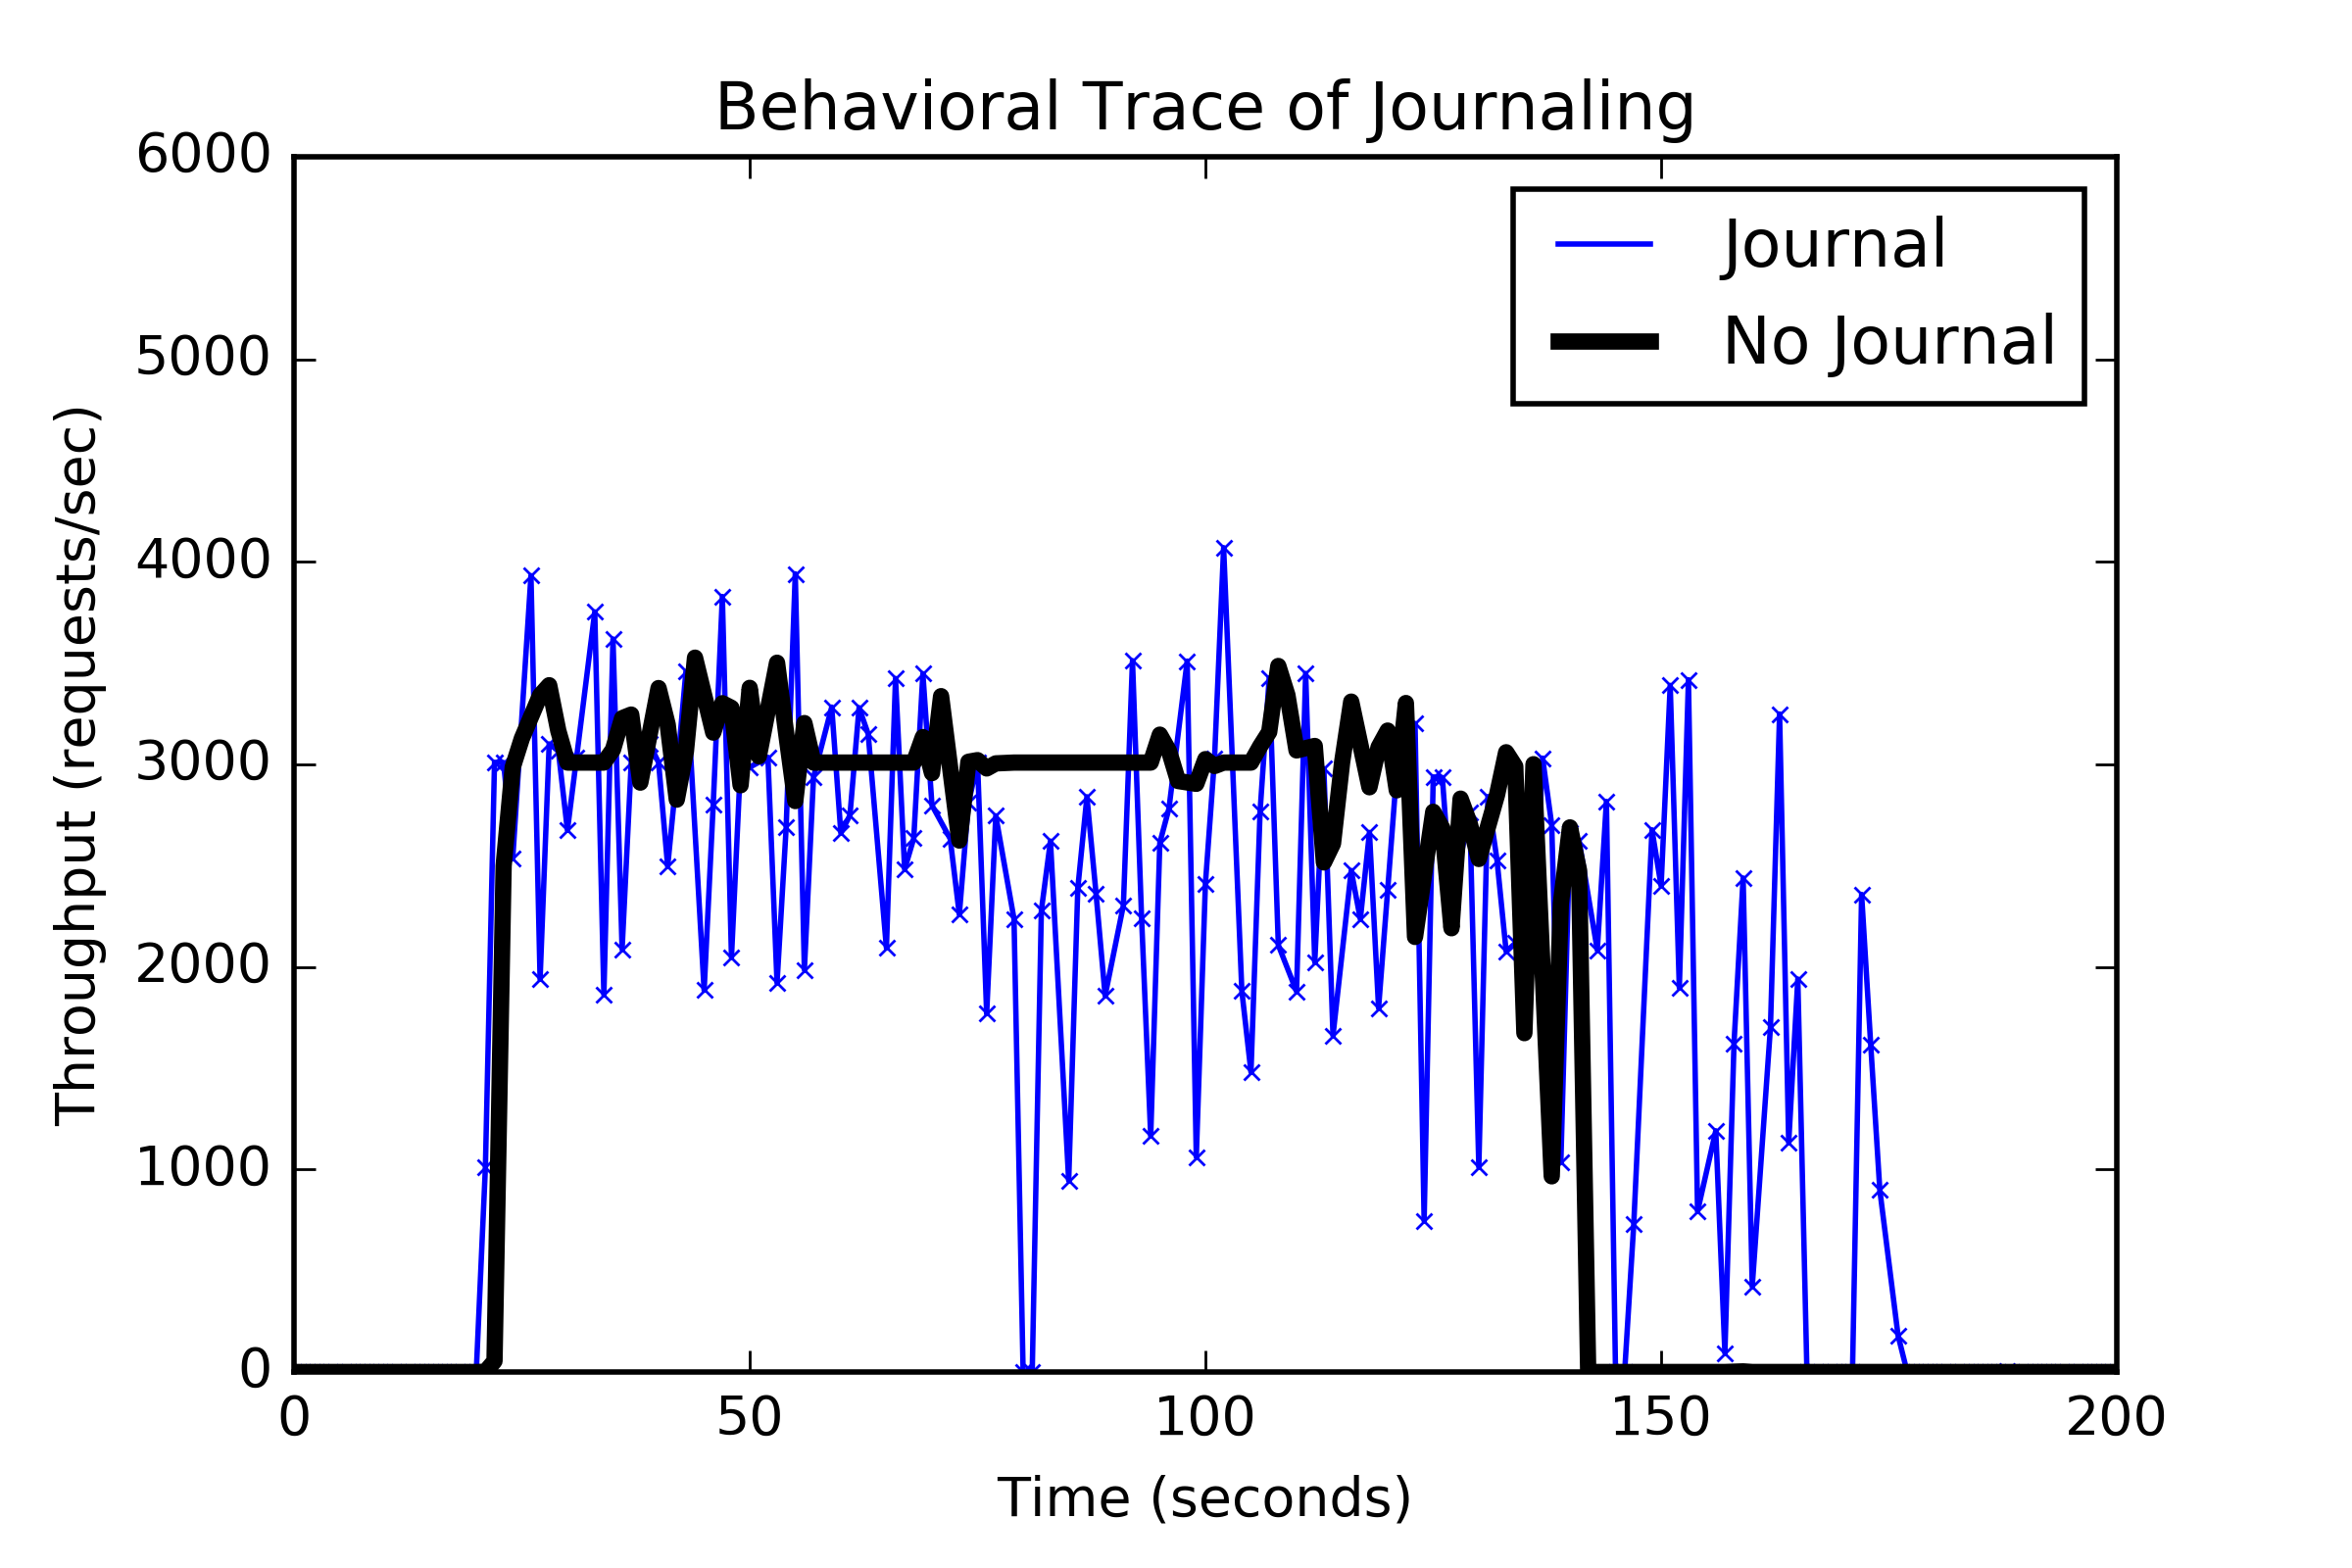
\includegraphics[width=1.0\linewidth]{graphs/behavior-journal.png}
      \caption{180MB Segment vs. No Journal}
      \label{fig:slowdown-journal-b}
  \end{subfigure}
  \begin{subfigure}[b]{.3\linewidth}
      \centering
      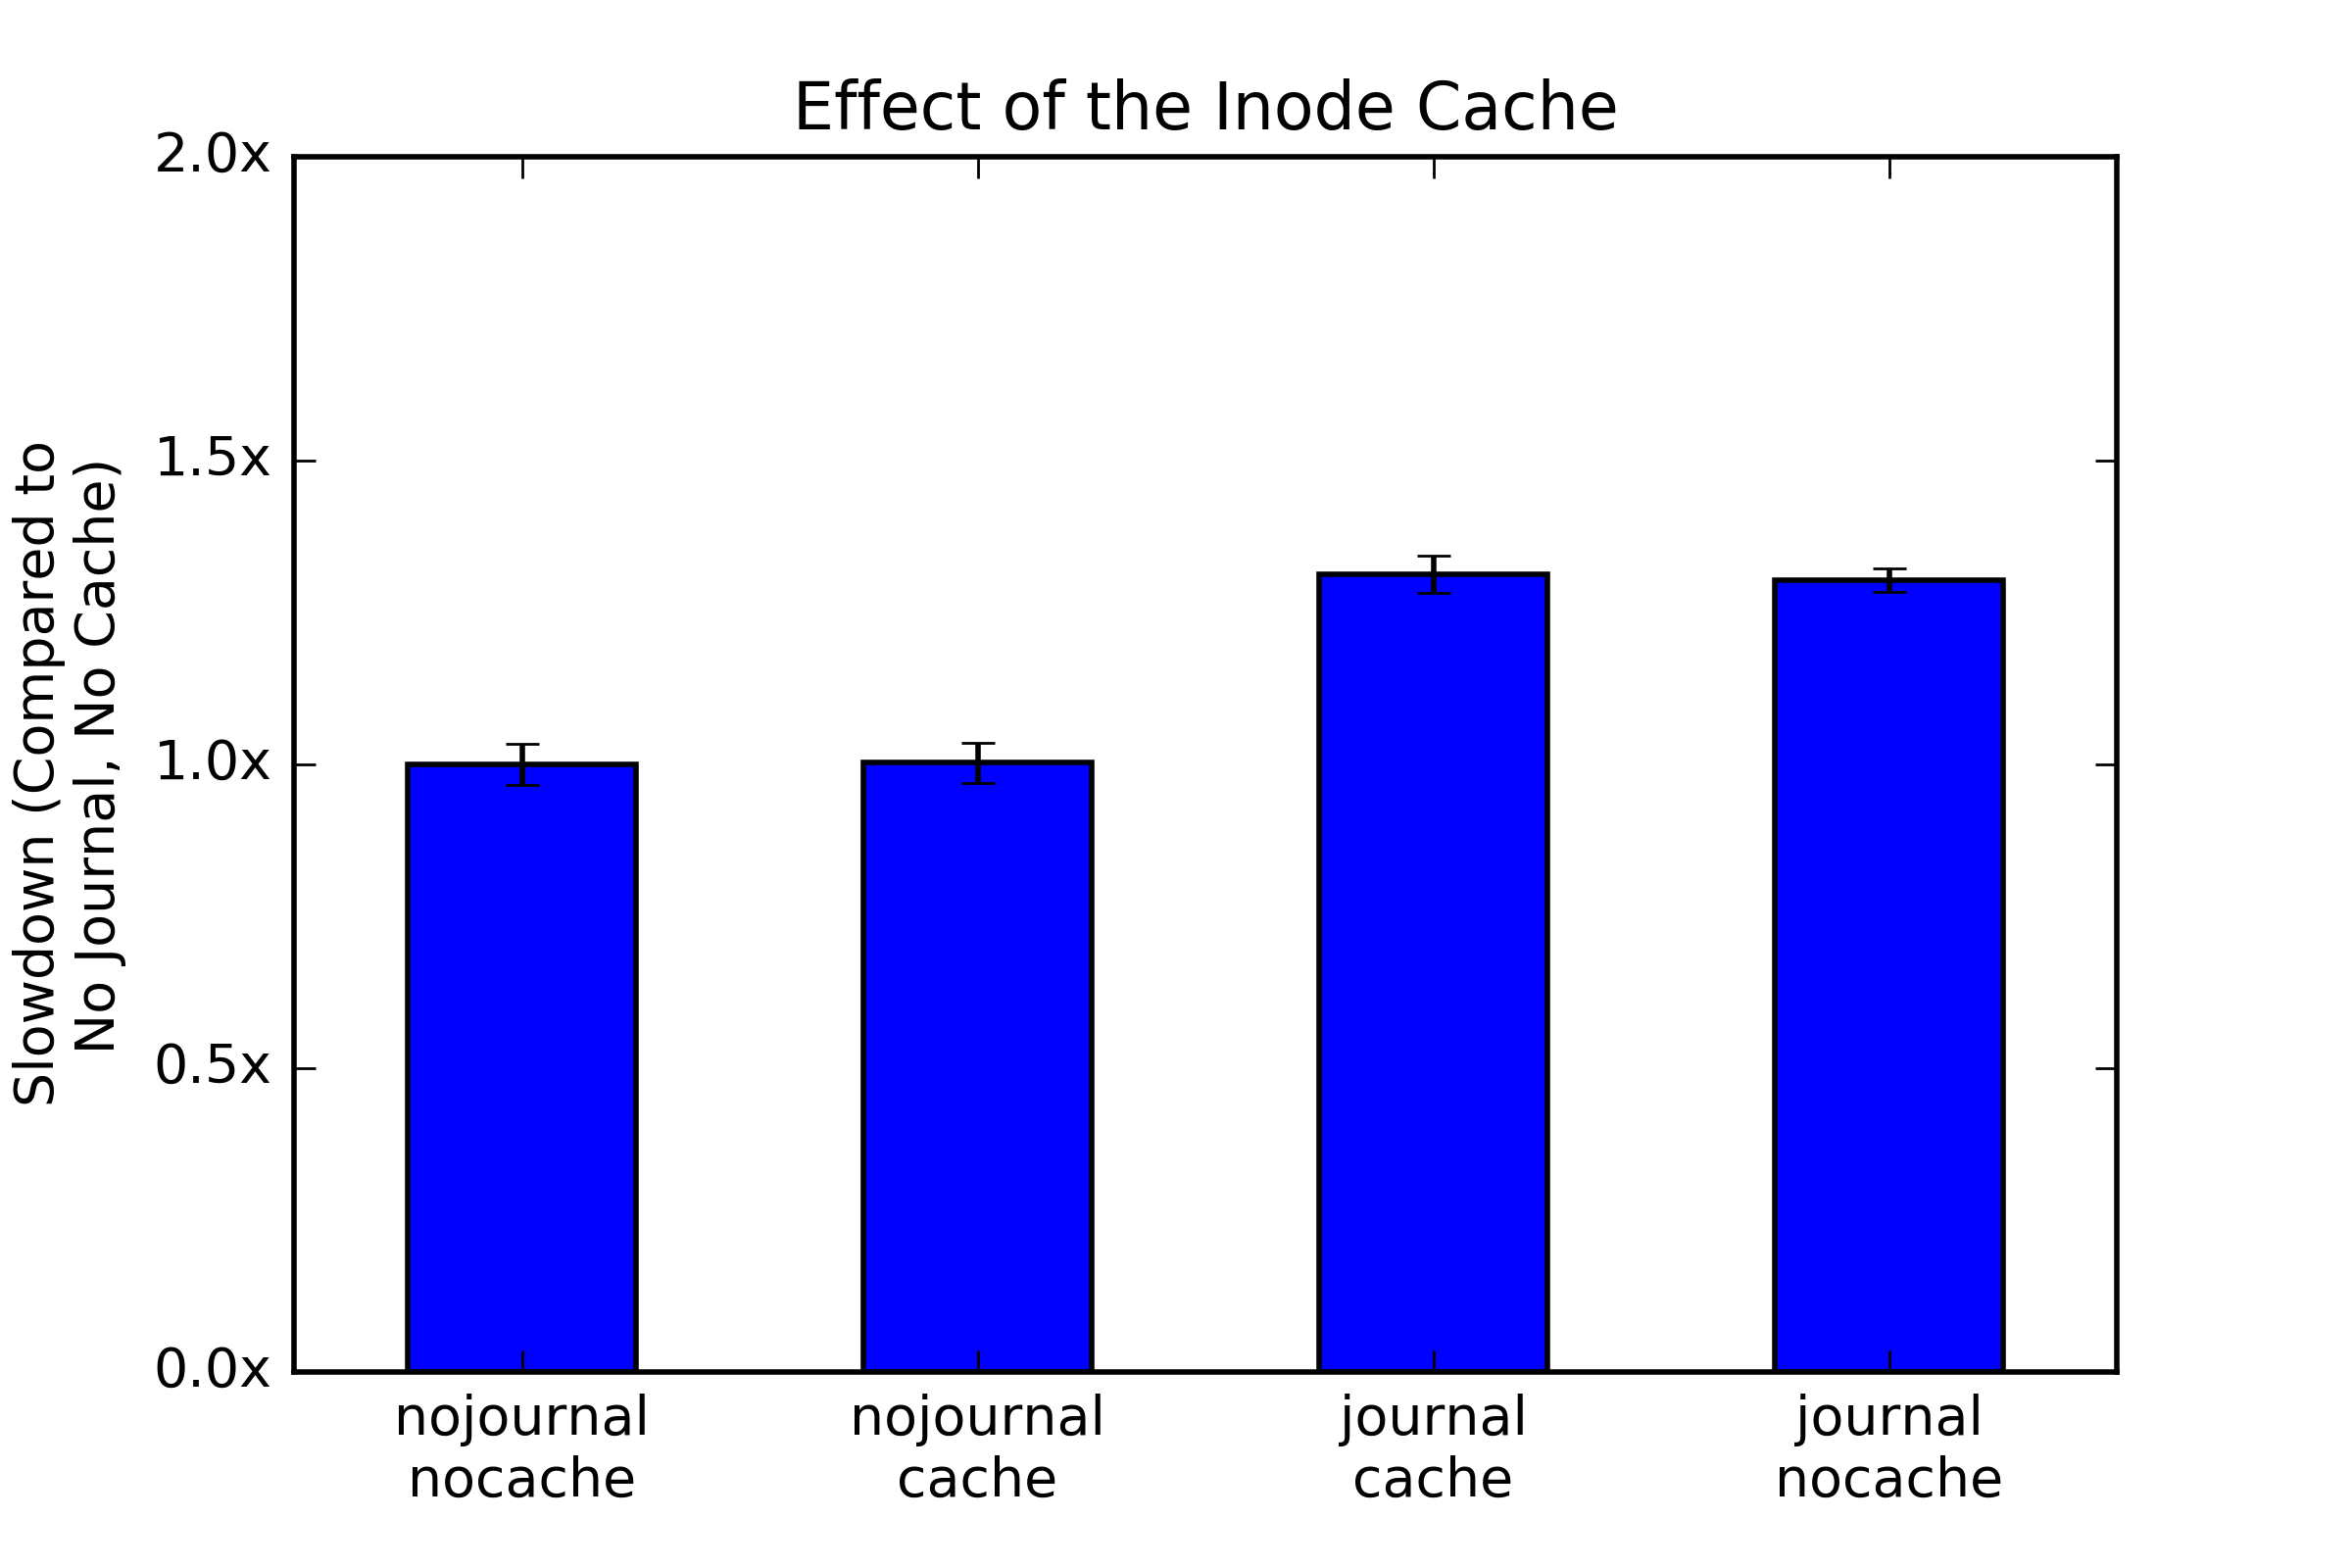
\includegraphics[width=1.0\linewidth]{graphs/slowdown-cache.png}
      \caption{Inode Cache}
      \label{fig:slowdown-journal-c}
  \end{subfigure}
  \caption{The overhead of the file system metadata journal. The segment size
  is the threshold that the metadata server starts
  trimming.\label{fig:slowdown-journal}}
\end{figure*}

% what is durability
While durability is not specified by POSIX, users expect that their metadata is
safe. We define three types of durability: global, local, and none.  Global
durability means that the client or server can fail at any time and metadata
will not be lost. Local durability means that metadata can be lost if the
client or server fails and stays failed. None means that metadata is volatile
and that the system provides no guarantees when clients or servers fail.\\

% - sequential IO, trim redundant operations
\noindent\textbf{CephFS Design}: a journal of metadata updates that streams into
the resilient object store. Similar to LFS~\cite{rosenblum:acm1992-LFS} and
WAFL~\cite{hitz:wtec1994-WAFL} the metadata journal can grow to large sizes
ensuring (1) sequential writes into RADOS and (2) the ability for daemons to
trim redundant or irrelevent journal entries.  The journal is striped over
objects where multiple journal updates can reside on the same object. There are
two tunables for controlling the journal: the segment size and the number of
parallel segments that can be written in parallel. The former is memory bound
as larger segments take up more memory but can reduce the time spent journaling
and the latter is CPU bound. 

% purpose of the journal
As shown in Figure~\ref{fig:journal}, in addition to the metadata journal,
CephFS also represents metadata in RADOS as a metadata store, where directories
and their file inodes are stored as objects.  The metadata server applies the
updates in the journal to the metadata store when the journal reaches a certain
size. The metadata store is optimized for recovery ({\it i.e.} reading) while
the metadata journal is write-optimized.

% Effects on performance
Figure~\ref{fig:slowdown-journal} shows that journaling metadata updates into
the object store has an overhead. Figure~\ref{fig:slowdown-journal-a} shows the
effect of journaling of different journal segment sizes; the larger the segment
size the bigger that the writes into the object store are. The trade-off for
better performance is memory consumption because larger segment sizes take up
more space with their buffers. Figure~\ref{fig:slowdown-journal-b} shows how
the metadata server periodically stops serving requests to flush ({\it i.e.}
apply journal updates to) the metadata store.  The journal overhead is
sufficient enough to slow down metadata throughput but not so much as to
overwhelm the bandidth of the object store. We measured our peak bandwidth to
be 100MB/s, which is the speed of our network link.\\

\noindent\textbf{Comparison to decoupled namespaces}: In BatchFS and DeltaFS,
as far as we can tell, when a client or server fails there is no recovery
scheme. For BatchFS, if a client fails when it is writing to the local
log-structured merged tree (implemented as an SSTable) then those batched
metadata operations are lost. For DeltaFS, if the client fails then on restart
the computation does the work again -- since the snapshots of the namespace are
never globally consistent and there is no ground truth.  On the server side,
BatchFS and DeltaFS use IndexFS. Again, IndexFS writes metadata to SSTables but
it is not clear whether they ever vacate memory, get written to disk, or are
flushed to the object store.

\subsection{Strong Consistency} 
\label{sec:strong-consistency}

Access to metadata in a POSIX-compliant file system is strongly consistent, so
reads and writes are globally ordered.  The synchronization and serialization
machinery needed to ensure that all clients see the same state has high
overhead.\\

\noindent\textbf{CephFS Design}: capabilities keep metadata strongly
consistent. To reduce the number of RPCs needed for consistency, clients can
obtain capabilities for reading, reading and updating, caching reads, writing,
buffering writes, changing the file size, and performing lazy IO.

\begin{figure*}[t]
  \centering
  \begin{subfigure}[b]{.3\linewidth}
      \centering
      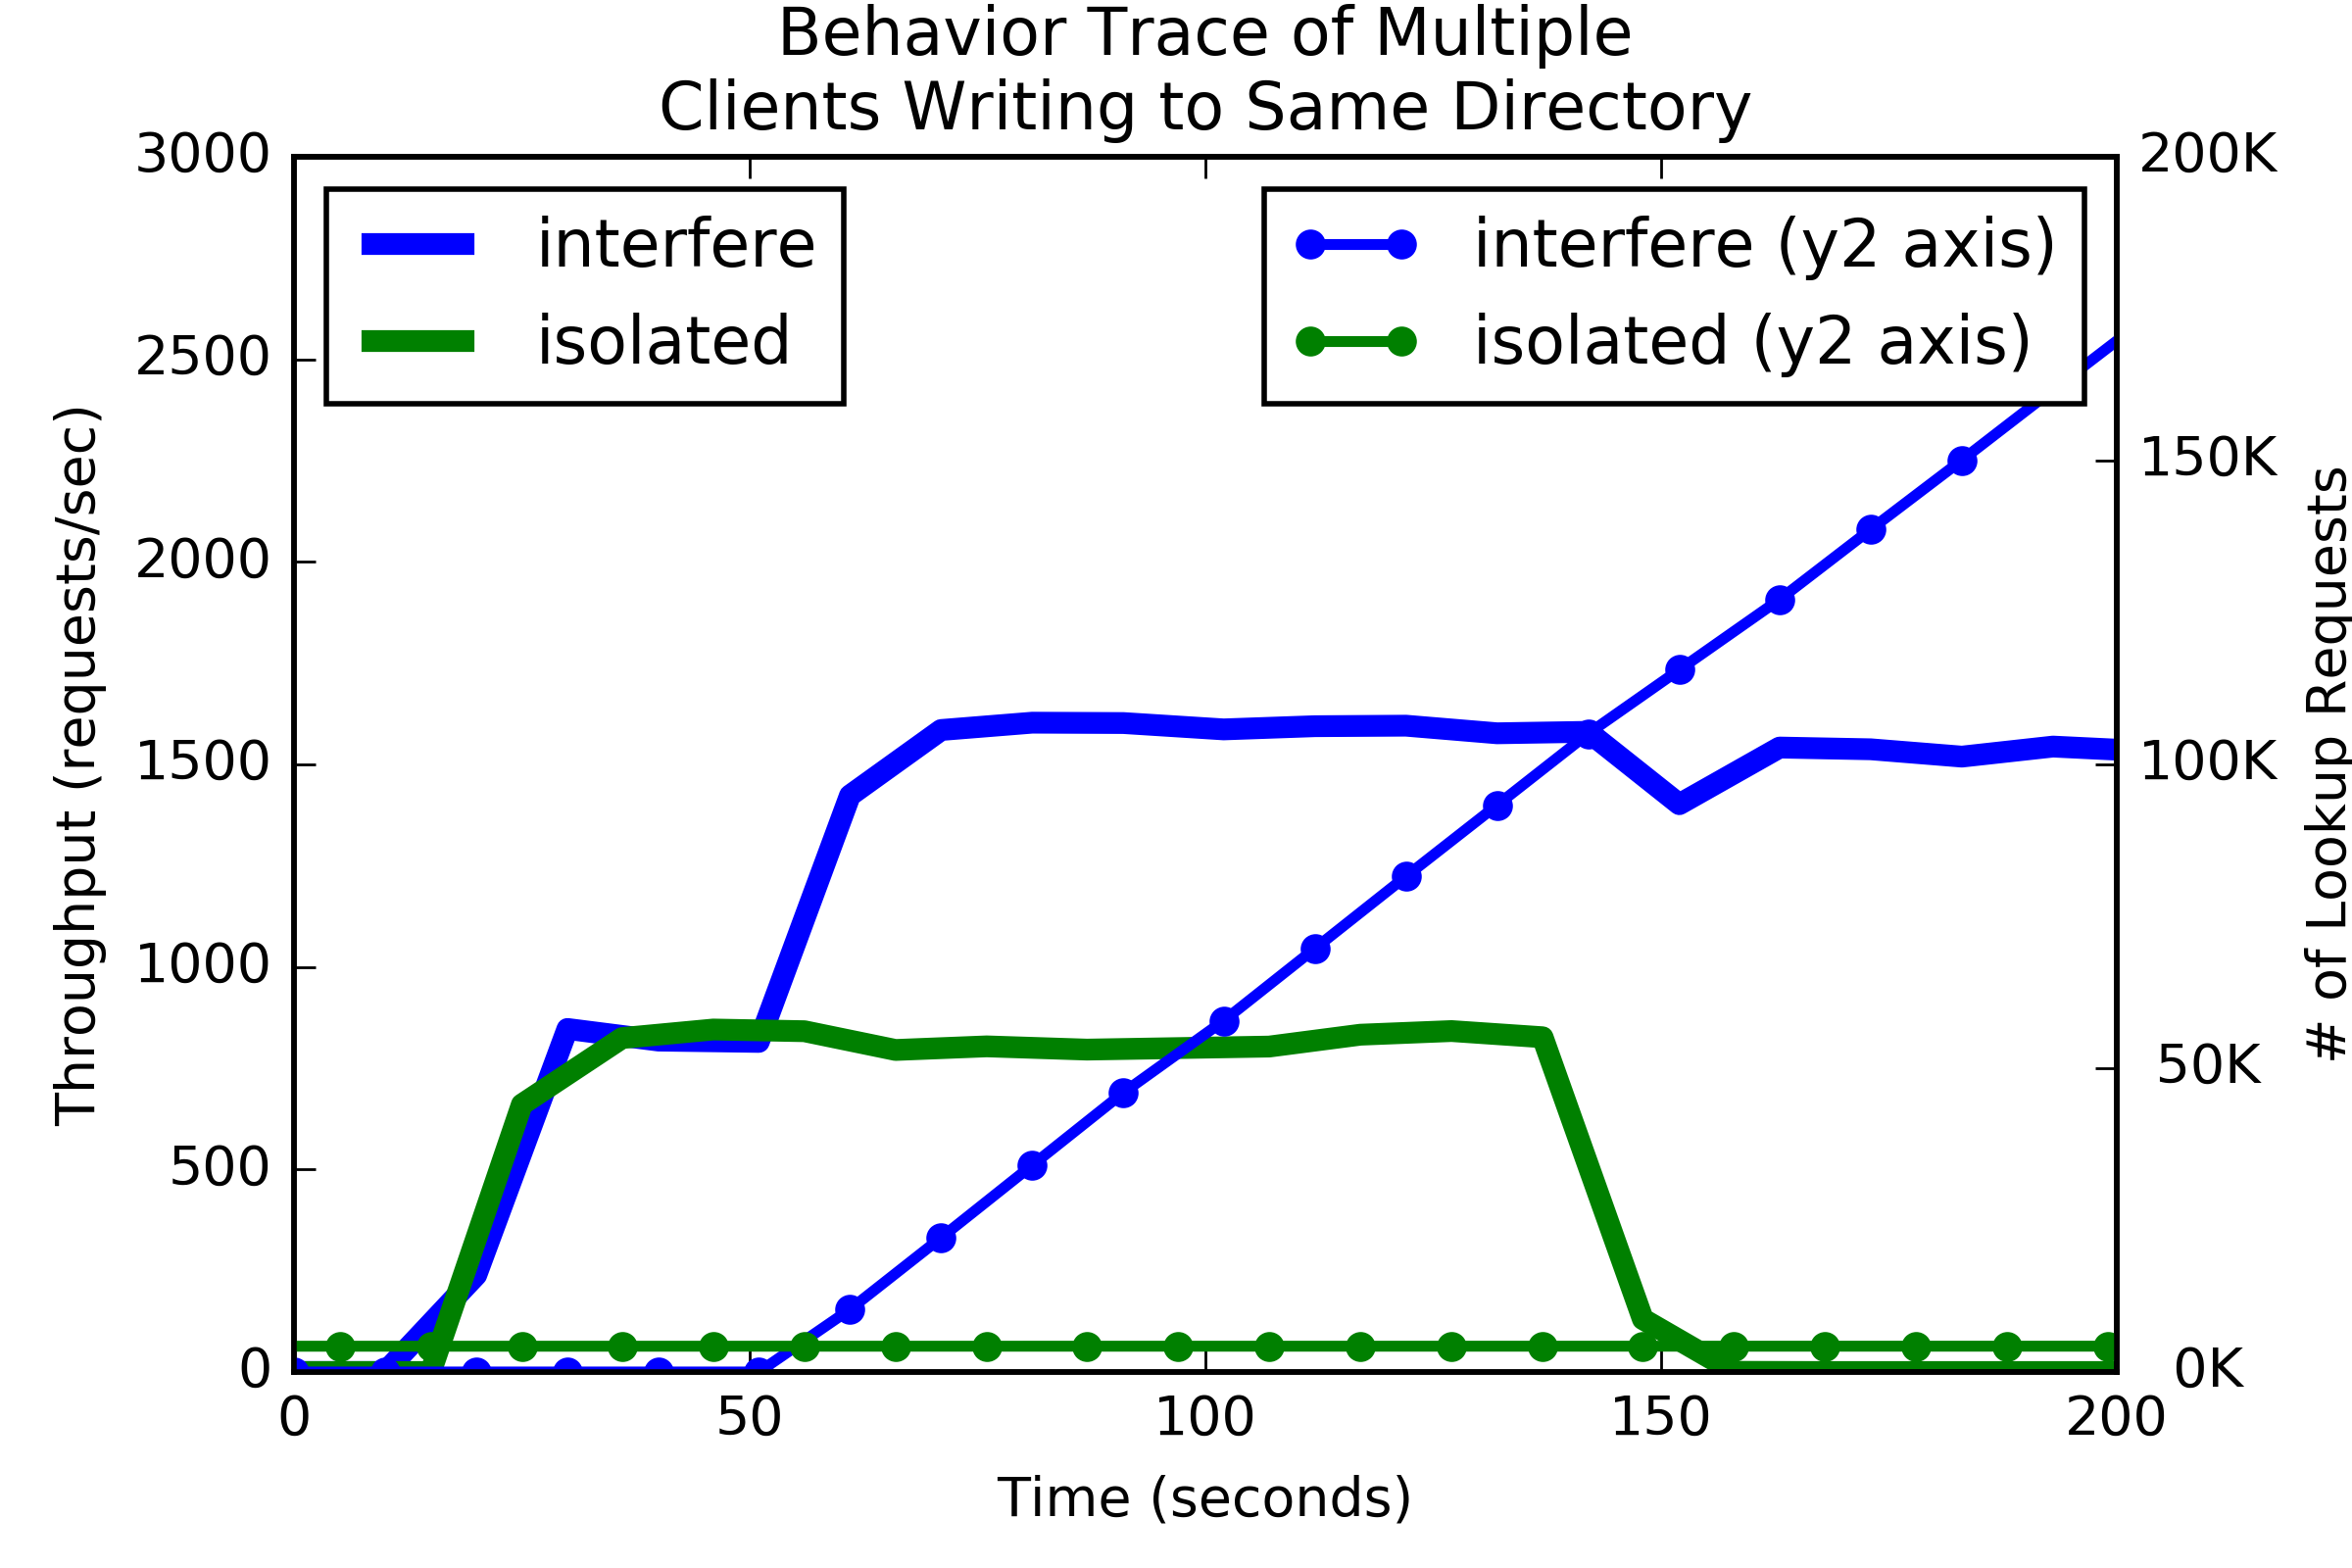
\includegraphics[width=1.0\linewidth]{graphs/behavior-interfere.png}
      \caption{Inteference forces \texttt{lookup()}s}
      \label{fig:interfere-a}
  \end{subfigure}
  \begin{subfigure}[b]{.3\linewidth}
      \centering
      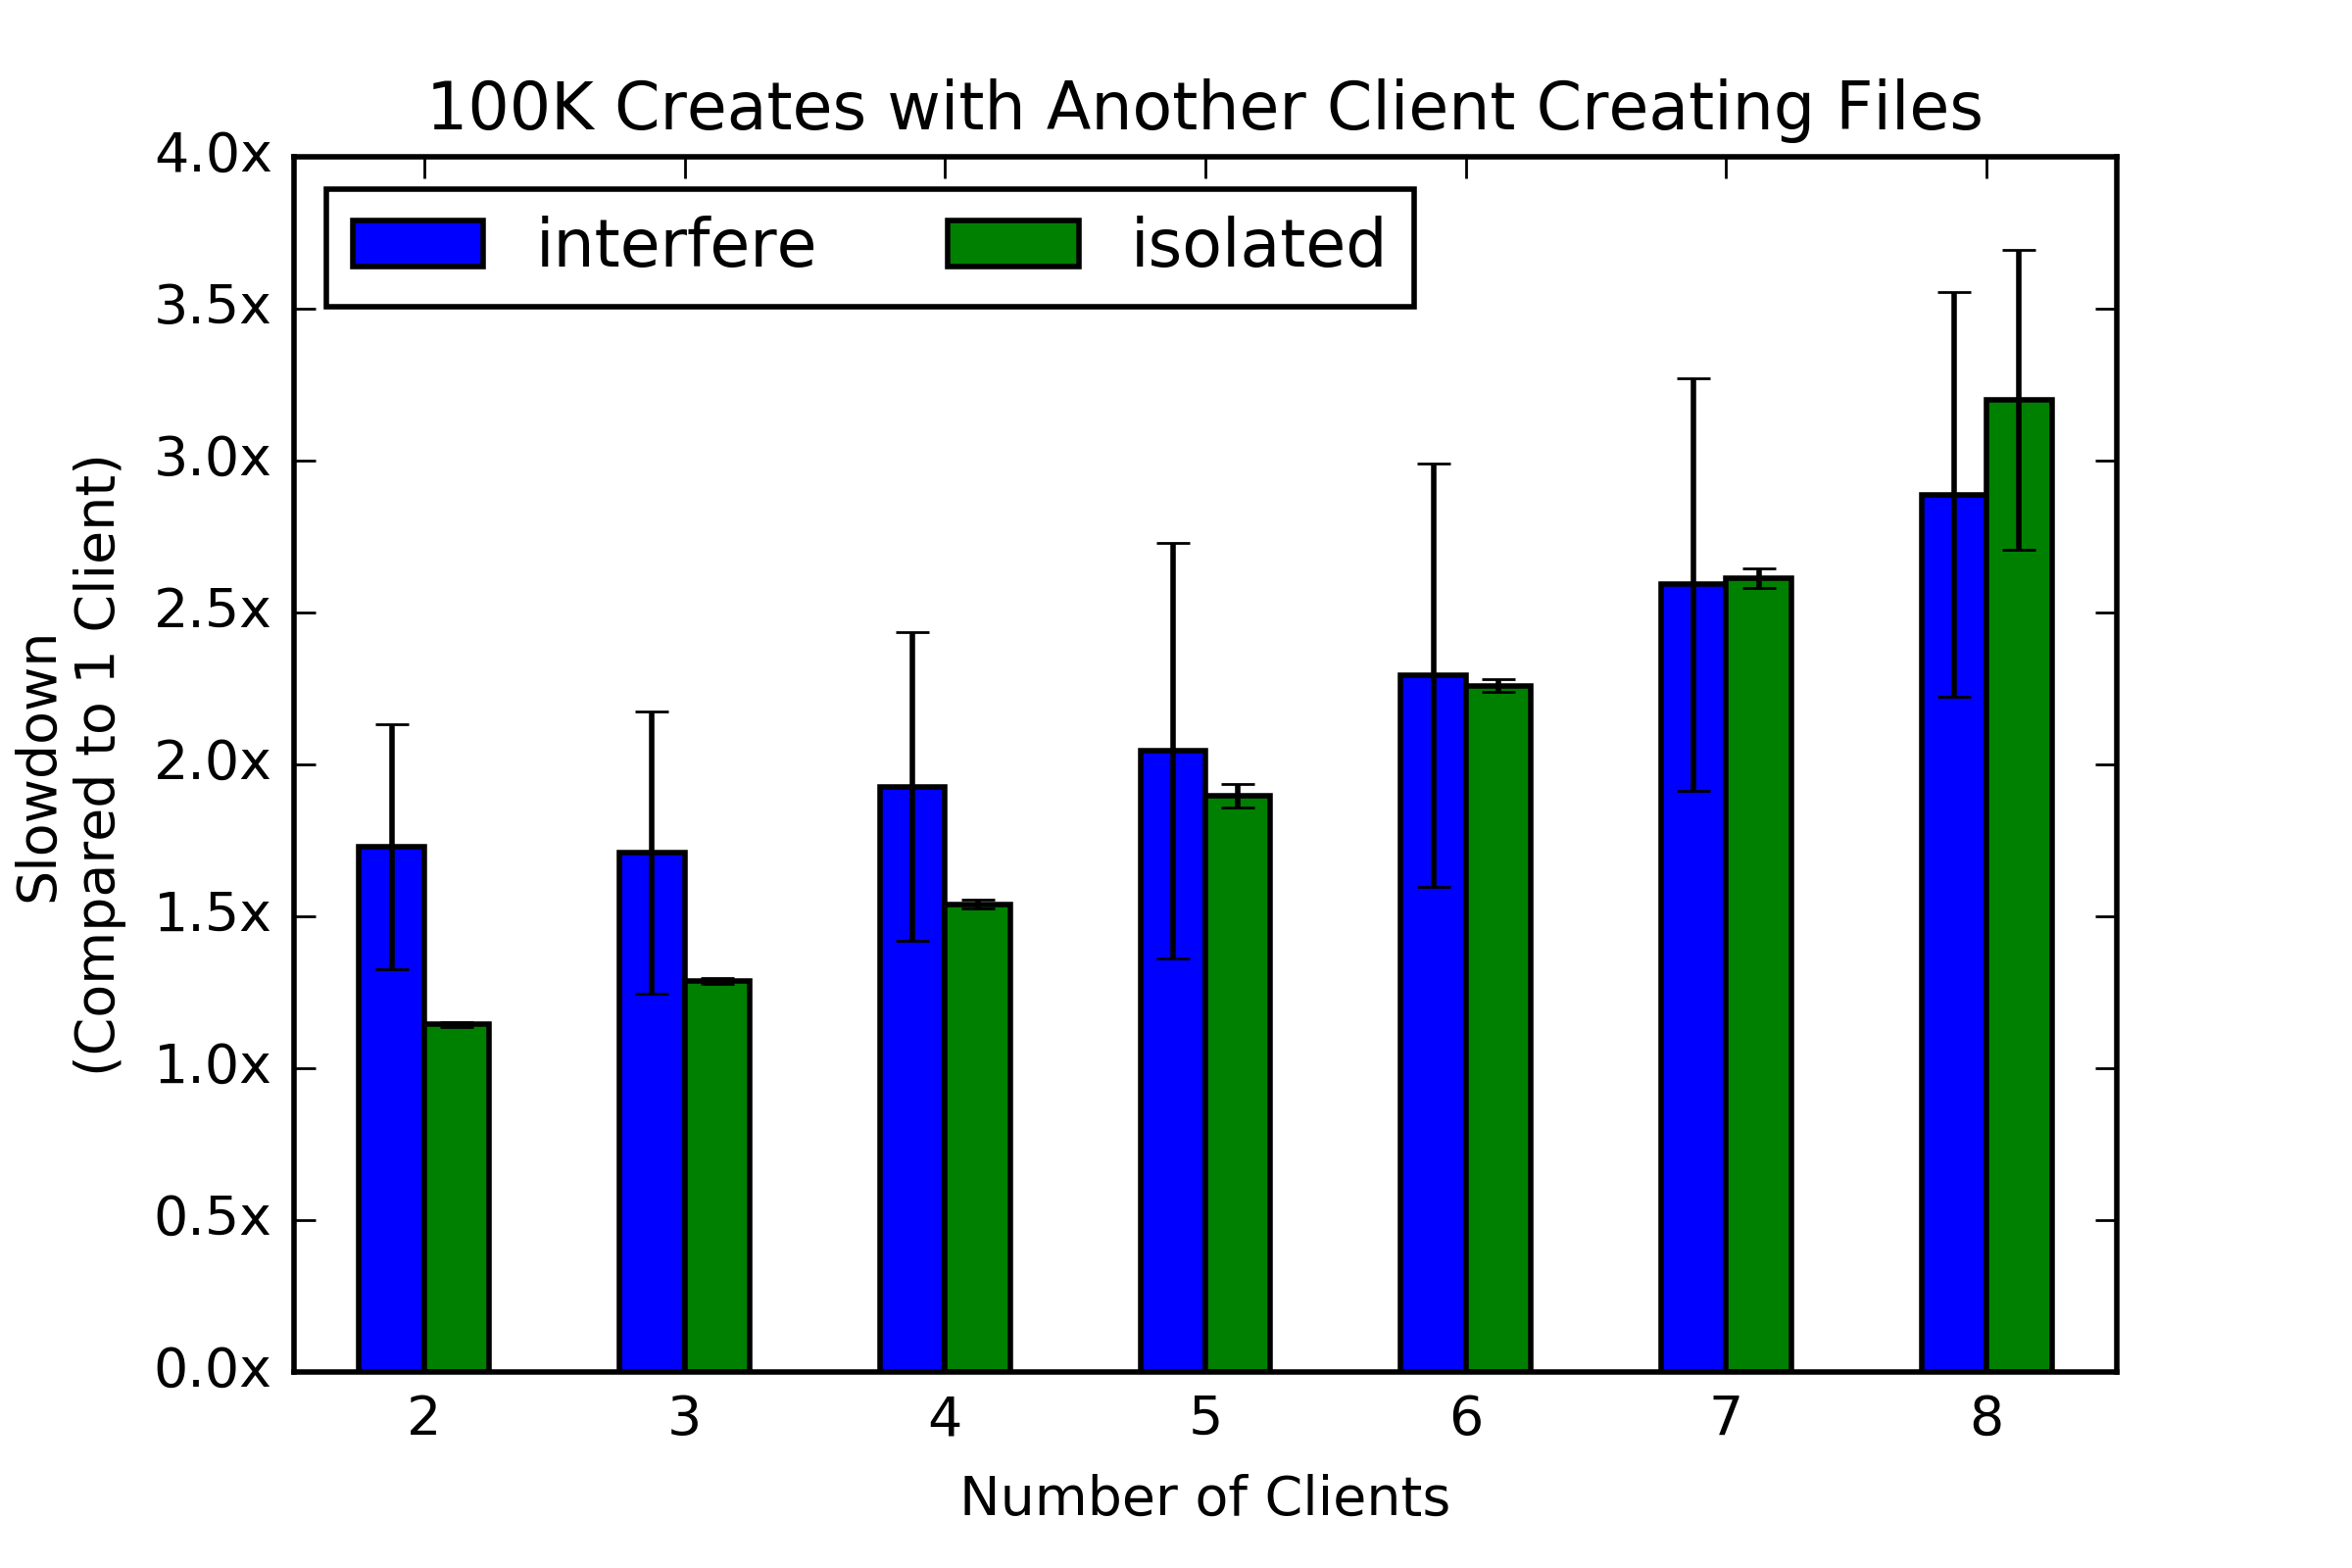
\includegraphics[width=1.0\linewidth]{graphs/slowdown-interfere.png}
      \caption{Interference hurts performance}
      \label{fig:interfere-b}
  \end{subfigure}
  \begin{subfigure}[b]{.3\linewidth}
      \centering
      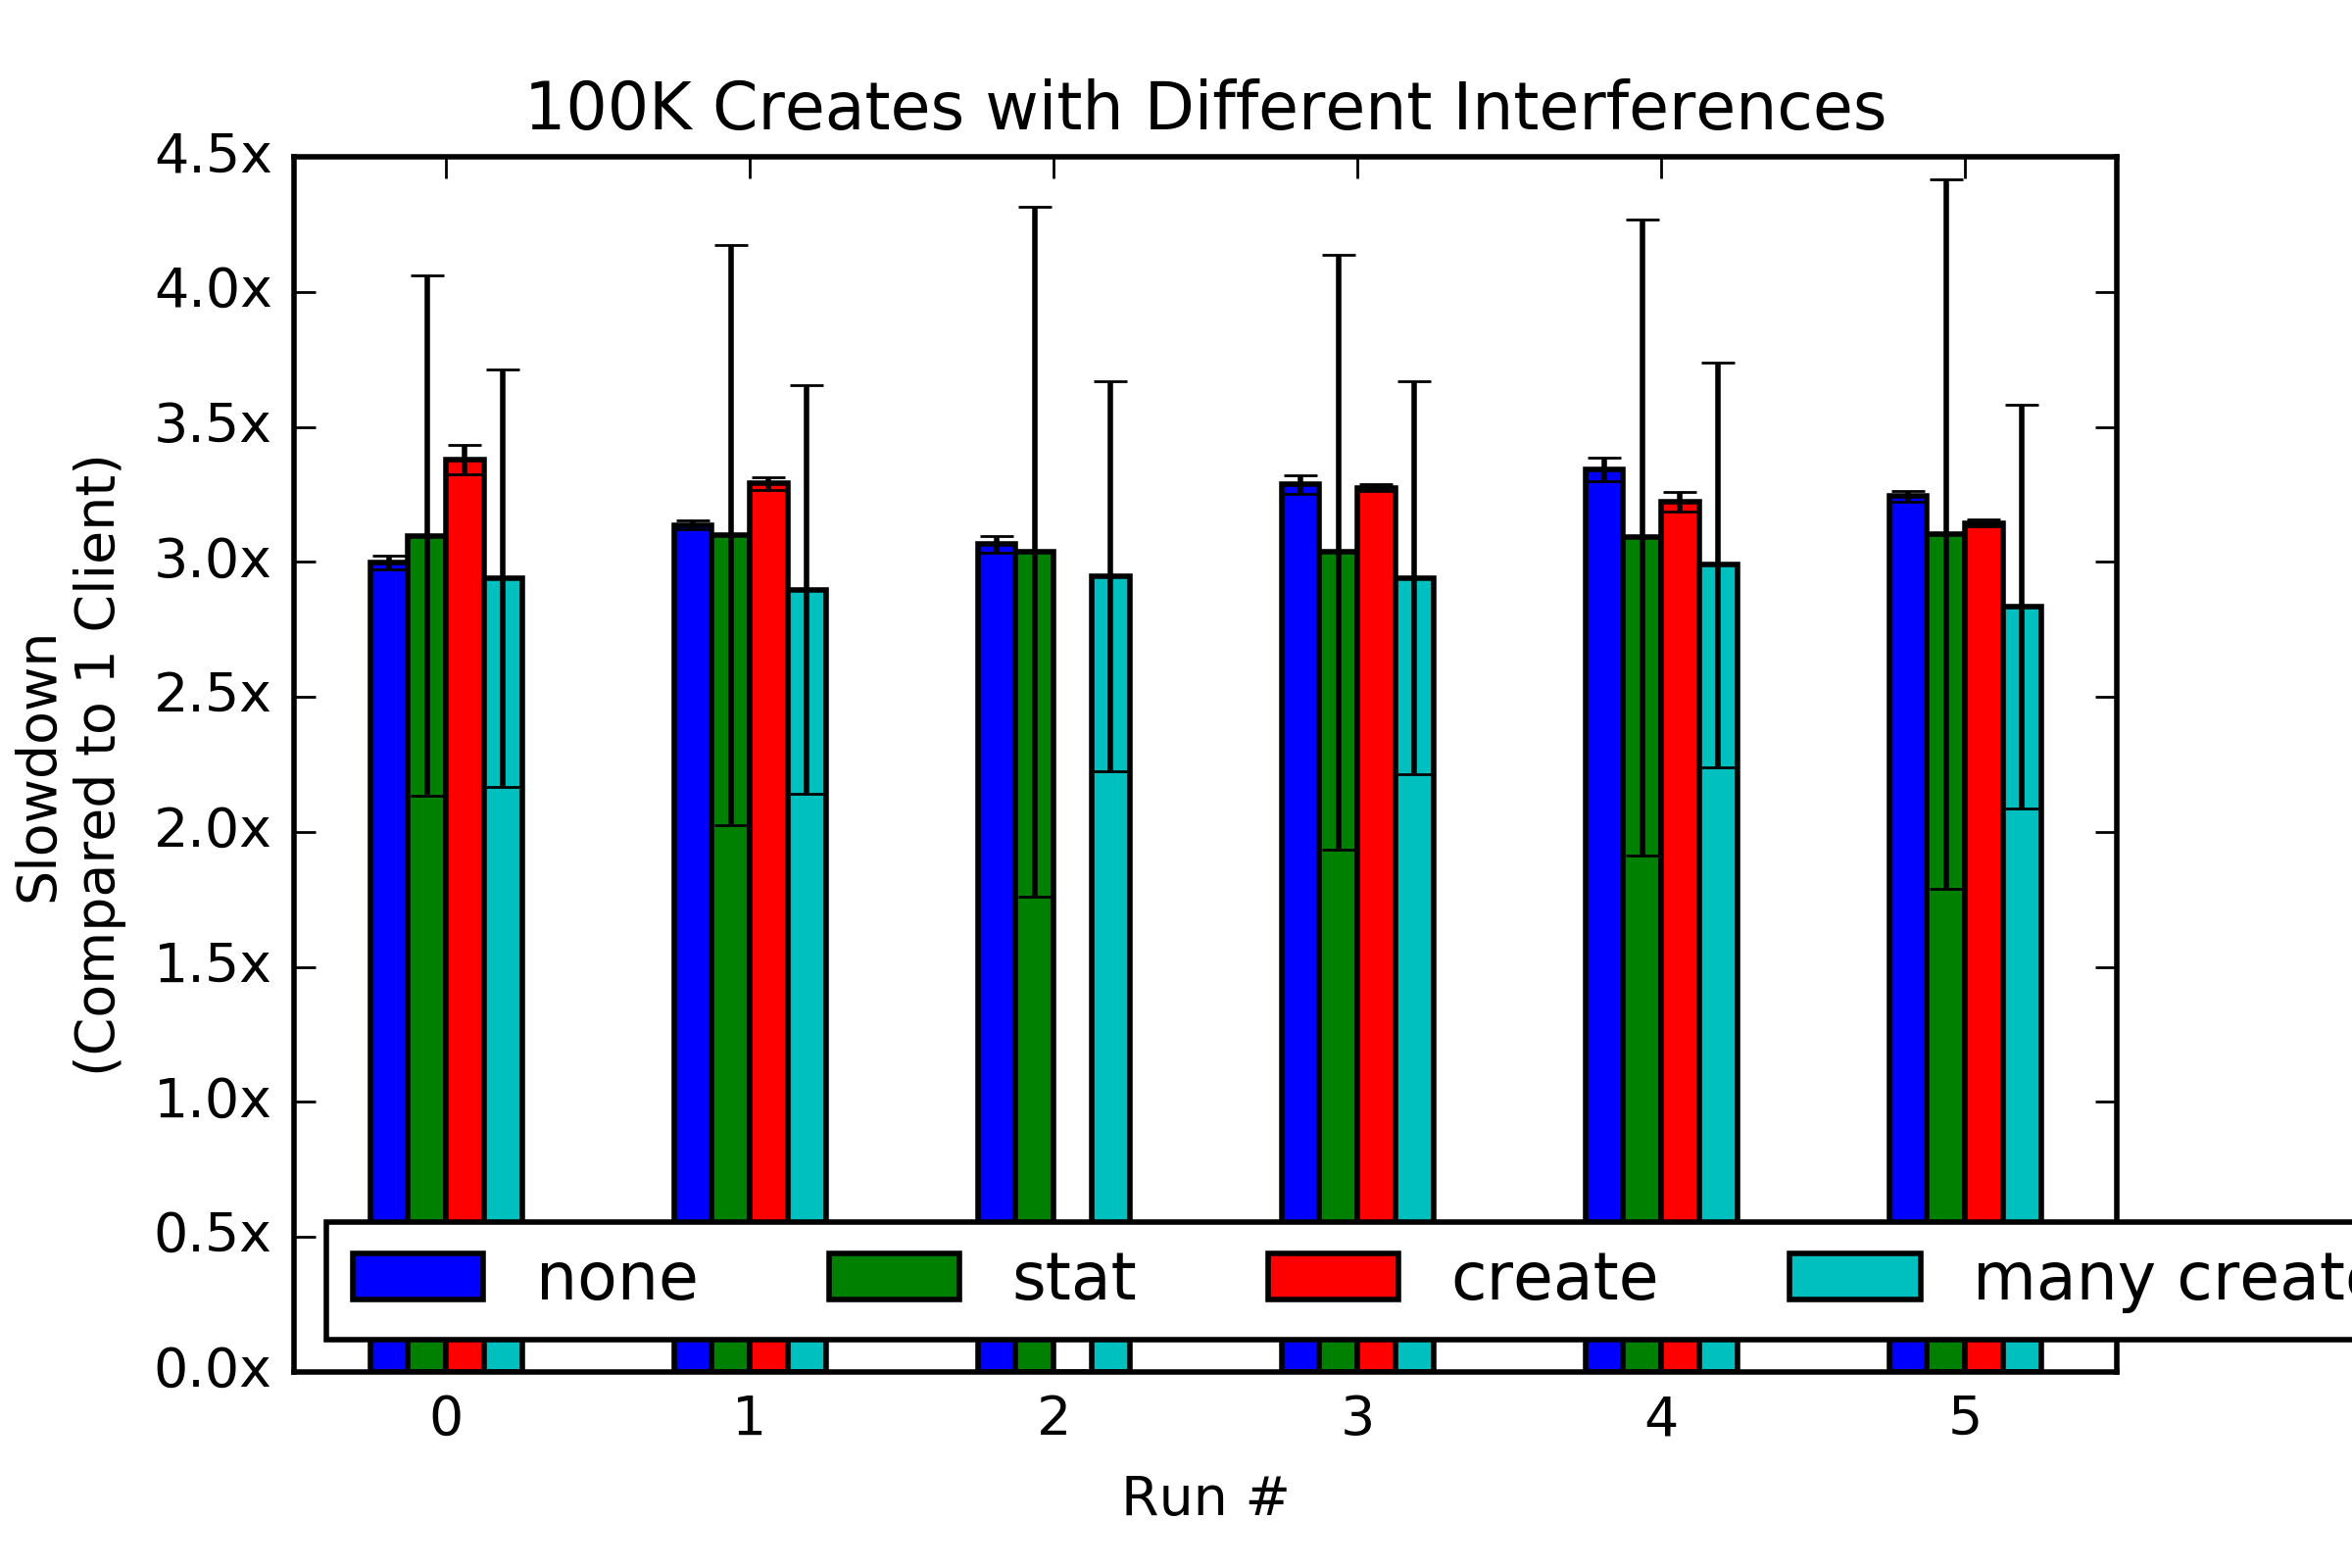
\includegraphics[width=1.0\linewidth]{graphs/slowdown-interfere-types.png}
      \caption{Different interferring requests}
      \label{fig:interfere-c}
  \end{subfigure}
  \caption{When a client create stream is ``isolated" then lookups resolve
  locally but when a second client ``interferes" by creating in the same
  directory, the directory inode capability is revoked forcing all clients to
  centralize lookups at the metadata server.  
  \label{fig:interfere}}
\end{figure*}

% inode cache - reduces RPCs (lookups for create, readdirs for stats)
To keep track of the read caching and write buffering capabilities, the clients
and metadata servers agree on the state of each inode using an inode cache.  If
a client has the directory inode cached it can do metadata writes ({\it e.g.},
create) with a single RPC. If the client is not caching the directory inode
then it must do an extra RPC to determine if the file exists.  Unless the
client immediately reads all the inodes in the cache ({\it i.e.} \texttt{ls
-alR}), the inode cache is less useful for create-heavy workloads.

% benefits PROBLEM -- IS THIS THE METADATA PROTOCOL OR JUST THE OVERLOADEDNESS?
The benefits of caching the directory inode when creating files is shown in
Figure~\ref{fig:interfere-a}.  If only one client is creating files in a
directory (``isolated" curve on \(y1\) axis) then that client can lookup the
existence of new files locally before issuing a create request to the metadata
server. If another client starts creating files in the same directory
(``interfere" curve on \(y1\) axis) then the directory inode transitions out of
read caching and the first client must send \texttt{lookup()}s to the metadata
server (``interfere" curve on \(y2\) axis). These extra requests increase the
throughput of the ``interfere" curve because the metadata server can handle the
extra load but the overall performance decreases.  This degradation is shown in
Figure~\ref{fig:interfere-b}, where we scale the number of clients and show
increased runtime and variability. The performance is compared to a single
isolated client and he error bar is the standard deviation of the runtime of
all clients.  For the ``interfere" bars, each client creates files in private
directories and at 30 seconds we launch another process that creates files in
those directories.  For less than 7 clients, the runtime and deviation is worse
when clients interfere. At 7 clients, the metadata server is overloaded so the
directory caching in the ``isolated" bars has no benefit. Zooming in on runs
with 7 clients in Figure~\ref{fig:interfere-c} we see how different
interferring operations affect performance, again when compared to the
performance of a single isolate client.  ``create" has little effect but
``stat" and ``create many" cause noticeable slowdowns because of the extra work
they impose on the metadata server.\\

% TODO: what is the cost of trimming the cache?
% TODO: does CephFS still cache inodes when I turn off caching? Why is still keeping inodes in memory? Gah!

\noindent\textbf{Comparison to decoupled namespaces}: Decoupled namespaces
merge batches of metadata operations into the global namespaces when the job
completes.  In BatchFS the merge is delayed by the application using an API to
switch between asynchronous to sychronous mode. The merge itself is explicitly
managed by the application but future work looks at more automated
methdologies. In DeltaFS snapshots of the metadata subtrees stays on the client
machines; there is no ground truth and consistent namespaces are constructed
and resolved at application read time or when a 3rd party system ({\it e.g.},
middleware, scheduler, etc.) needs a view of the metadata. As a result, all the
overheads of maintaining consistency that we showed above are delayed until the
merge phase.

\section{Methodology: Decoupled Namespaces}
\label{sec:methodology-decoupled-namespaces}

\begin{figure}[tb]
\caption{Applications can decouple the namespace, write updates to a local
journal, and delay metadata updates.  Table~\ref{table:spectrum} shows how
these mechanisms (represented by the arrows) can be combined to provide weaker
consistency or durability semantics.  }\label{fig:decouple}
\centering
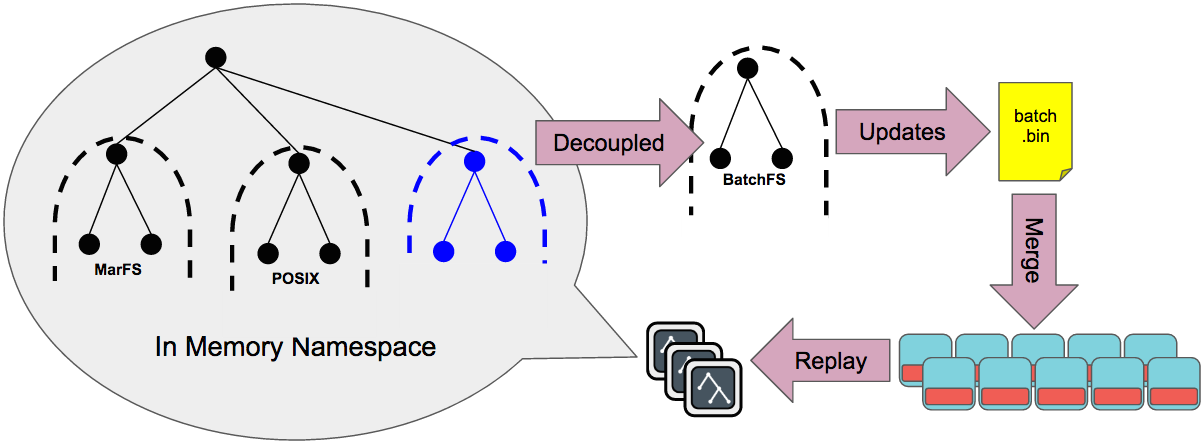
\includegraphics[width=90mm]{figures/fig-decouple.png}
\end{figure}

In this section we describe Cudele, our prototype system that lets future
programmers compose mechanisms (Section~\S\ref{sec:cudeles-mechanisms}) to
provide the necessary guarantees
(Section~\S\ref{sec:setting-policies-with-cudele}) for their application.

\subsection{Cudele's Mechanisms}
\label{sec:cudeles-mechanisms}

% describe the figure
Figure~\ref{fig:decouple} shows the mechanisms (labeled arrows) in Cudele and
which entity they are performed by (gray boxes). The metadata store and journal
are different ways of representing the namespace. The metadata store represents
the namespace as a tree of directory fragments and is easier to read/traverse.
The journal represent the namespace as a list of events. It is
a ``pile system"; writes are fast but reads are slow because state must be
reconstructed.  Specifically, reads are slow because there is more data to
read, it is unorganized, and many of the updates may be redundant.

% describe the mechanisms
Cudele presents 6 mechanisms: RPCs, Stream, Create, Volatile Apply, Local Persist, and Global
Persist. ``RPCs" does round trip remote procedure calls to establish
consistency; it is the default implementation for complying with POSIX in
CephFS. ``Stream" has the metadata servers stream a journal of metadata updates
into the object store. ``Create" allows clients to append metadata events to an
in-memory journal. ``Volatile apply" takes the in-memory journal on the client
and applies it directly to the in-memory metadata store of the metadata server
cluster. ``Local Persist" takes the in-memory journal and writes it to the client's
disk. ``Global Persist" saves the journal as a an object in the object store from the
client.

Next, we discuss how these mechanisms can be composed to get different
consistency and durability semantics. 

%\begin{tabular}{ r | l }
%  \(\Rightarrow\)   & Description \\\hline
%  create            & events appended to in-memory journal \\
%  v\_apply           & journal volatily applied to in-memory metadata store \\
%  save              & journal saved to client's disk \\
%  persist           & journal saved in object store \\
%  replay            & metadata servers materialize namespace \\
%  RPCs              & round trip remote procedure calls \\
%  stream            & metadata server streams journal into RADOS \\
%\end{tabular}

\subsection{Setting Policies with Cudele}
\label{sec:setting-policies-with-cudele}

\begin{table}[t]
\begin{center}
\caption{Future programmers can explore the consistency (C) and
durability (D) spectrums by composing Cudele mechanisms. The consistency
and durability properties are not guaranteed until all mechanisms in the cell
are complete ({\it i.e.} the compositions should be considered atomic) and there are
no guarantees while tranisitioning between policies. \label{table:spectrum}}
\begin{tabular}{ l | l | l | l }
  C \(\rightarrow\) &&& \\  
  D \(\downarrow\)  	     & invisible         & eventual        & strong  \\\hline
  none                       & create            & create          & RPCs    \\
                             &                   & +volatile apply &         \\\hdashline
  local                      & create            & create          & RPCs    \\
                             & +local persist    & +local persist  & +local  \\
                             &                   & +volatile apply &  persist\\\hdashline
  global                     & create            & create          & RPCs    \\
                             & +global persist   & +global persist & +stream \\
                             &                   & +volatile apply &         \\
\end{tabular}
\end{center}
\end{table}

% describe table
The spectrum of consistency and durability guarantees that adminstrators can
construct is shown in Table~\ref{table:spectrum}. The columns are the different
consistency semantics and the rows cover the spectrum of durability guarantees.
For consistency: ``invisible" means the system does not handle merging updates
into a global namespace and it is assumed that middleware or the application
manages consistency lazily; ``eventual" merges updates at some time in the
future ({\it e.g.}, when the system has time, when number of updates reaches a
certain threshold, when the client is done writing, etc.); ; and updates in
``global" consistency are seen immediately by all clients. For durability,
``none" means that updates are volatile and will be lost on a failure. Stronger
guarantees are made with ``local", which means updates will be retained if the
client node recovers, and ``global", where all updates are always recoverable.

% which system they represent and which are impossible
Existing, state-of-the-art systems in HPC can be represented by the cells in
Table~\ref{table:spectrum}.  POSIX-compliant systems like CephFS and IndexFS
have global consistency and durability; DeltaFS uses ``invisible" consistency
and ``local" durability and BatchFS uses ``eventual" consistency and ``local"
durability. These are just a few of the HPC examples.  

% how its done
To compose the mechanisms administrators inject which steps (described in
Section~\S\ref{sec:cudeles-mechanisms}) to run and which to use in parallel
using a domain specific language. For example, to get the semantics of BatchFS,
the administrator would inject the following pipeline:\\

\noindent \texttt{create+save+volatile apply}\\

% what is impossible
Although we can achieve all permutations of the different guarantees in
Table~\ref{table:spectrum}, not all of them make sense. For example, it
makes little sense to do \texttt{creates+RPCs} since both steps do the same
thing or \texttt{stream+save} since ``global" durability is stronger and has
more overhead than ``local" durability.  Formulaically, valid steps
include:\\

\noindent \texttt{<create|RPCs> [+v\_apply][+save][+persist][+stream]}

\subsection{Cudele Namespace API:\\Per-Subtree Policies}
\label{sec:cudele-namespace-api-per-subtree-policies}

% the interface
The interface for setting the subtree policies is with \{path,
\(<\)block\(|\)overwrite\(>\), pre-allocated inodes\} tuples. For example:

\texttt{(msevilla/mydir, policies.yml)}

would decouple the path \texttt{msevilla/mydir} and would apply the policies in
\texttt{policies.txt}. The policies file supports the following values:

\begin{itemize}

  \item \texttt{allocated\_inodes}: the number of inodes to allocate to the
  decoupled namespace (default 100)

  \item \texttt{interfere\_callback}: how to handle a request from another
  client targeted at the now decoupled subtree (default \texttt{block})

  \item \texttt{consistency\_callback}: which consistency model to use (default
  \texttt{RPCs})

  \item \texttt{durability\_callback}: which durability model to use (default
  \texttt{stream})

\end{itemize}

Given these default values decoupling the namespace with an empty policies file
would give the application 100 inodes but the subtree would behave like the
existing CephFS implementation. Table~\ref{table:spectrum} shows how one would use the Cudele
API to implement policies from related work. 


%

For \texttt{block}, any requests to this part of the namespace returns with
``Device is busy", which will spare the metadata server from wasting resources for updates
that may get overwritten. If the application does not mind losing updates, for
example it wants approximations for results that take too long to compute, it
can select \texttt{overwrite}. In this case, metadata will be written and the
computation from the decoupled namespace will take priority at merge time because the results
are more accurate.

\begin{listing}
\begin{minted}[frame=single,
               framesep=3mm,
               xleftmargin=21pt,
               tabsize=4]{js}
{     
    "allocated_inodes": "100000"
    "interfere_policy": "block"
    "consistency": "create"
    "durability": "local_persist"
}
\end{minted}
\caption{Implementing DeltaFS with Cudele.}
\label{src:deltafs}
\end{listing}

\begin{listing}
\begin{minted}[frame=single,
               framesep=3mm,
               xleftmargin=21pt,
               tabsize=4]{js}
{     
    "allocated_inodes": "100000"
    "interfere_policy": "block"
    "consistency": "create+volatile_apply"
    "durability": "local_persist"
}
\end{minted}
\caption{Implementing BatchFS with Cudele.}
\label{src:batchfs}
\end{listing}

\begin{listing}
\begin{minted}[frame=single,
               framesep=3mm,
               xleftmargin=21pt,
               tabsize=4]{js}
{     
    "allocated_inodes": "-"
    "interfere_policy": "-"
    "consistency": "RPCs"
    "durability": "stream"
}
\end{minted}
\caption{Existing CephFS on Cudele.}
\label{src:batchfs}
\end{listing}

\subsection{Programmability Approach}

% what is programmability
A programmable storage system exposes internal subsystem as building blocks for
higher level services. This `dirty-slate' approach limits redundant code and
leverages the robustness of the underlying storage system. Cudele uses this
approach and re-uses some of the building blocks from the Malacology
programmable storage system~\ref{sevilla:eurosys17} to great success and
requires only:

\begin{itemize}

  \item 354 lines of library code

  \item 219 lines of non-destructive metadata server code, which is not used
  unless it is turned on

  \item 4 lines of destructive client/server code to check whether a namespace
  is decoupled

\end{itemize}

% how it works in CephFS, how I used it
\subsubsection{Metadata Store}

\subsubsection{Journal}

\subsubsection{Journal Tool}
The journal tool is used for disaster recovery and lets administrators view and
modify the journal of metadata updates; it can read the journal, erase events
from the journal, and apply the updates in the journal to the metadata store.
To apply journal updates to the metadata store, the journal tool reads the
journal segments from object store objects and applies the update to the
metadata store (which are also stored as object store objects).  

% Journal import
The journal tool imports journals from binary files stored on disk.  First the
header of the dump is sanity checked and written into RADOS to the ``header"
object.  The ``header" object has metadata about the journal as well as the
locations of all the journal pointers (e.g., where the tail of the journal is,
where we are currently trimming, etc.).  Then the journal events are cleaned
(erasing trailing events that are not part of the header) and written as
objects into RADOS.  Note that while the journal is in RADOS, the metadata
servers do do not have the namespace reconstructed in memory so the metadata
cluster will not service requests relating to the journal of imported events.
To construct the namespace in the collective memory of the metadata servers we
need to first construct the namespace in RADOS. The journal tool can explicitly
do this by  applying the journal to the metadata store in RAODS. This will pull
the objects containing journal segments and replay them on the metadata store.
Finally, we delete the journal in RADOS and restart the metadata servers so
they rebuild their caches.

% Journal export
The journal tool exports journals to binary files stored on disk. First the
journal is scanned for the header and then journal is recovered. To recover the
journal the ``header" object is read off disk and then objects are probed in
order and starting from the write position saved in the header. Probing will
update the write position if it finds objects with data in them. 

% Journal export
When exporting a journal of events, the journal tool first scans the journal to
check for corruption. Then it recovers the journal by reading the ``header"
object out of RADOS.  After reading the header, the journal tool can pull
journal segments from RADOS because it knows how many objects to pull and how
far to seek within those objects.

%% The data structures
%The metadata that the event touches, including inodes, paths, and timestamps,
%are stored as metablobs. Each piece of metadata inside a metablob is called a
%dirlump. A dump has a section for lumps (dirfrag, dirlump), roots (dentries),
%table client transactions (tid, version), renamed directory fragments (maps,
%versions, alloc/preallocated inodes), inodes starting a truncate, inodes
%finishing a truncate, destroyed inodes, and client requests. Unfortunately for
%me (and you since you are reading this paper), this does not make any sense.
%
%Each directory fragment has an associated directory lump, which is just a bunch
%of metadata. The most interesting part of the dirlump is the fullbits array,
%which has a dentry OR inode. To walk the tree, iterate over all the dirlumps
%and then all the full bits, saving off the children and inode locations. The
%children tell us which dentry names an inode has and the inode locations map
%the parent inode to its child inode and dentry.  



\subsubsection{Inode Cache}

\subsubsection{Large Inodes}

% file type
To assign consistency and durability to the subtrees we store policies in
the directory inode. This approach uses the File Type interface from the
Malacology programmable store system~\cite{sevilla:eurosys17} and it tells clients how to access
the underlying data or metadata. The underlying implementation stores
executable code in the inode that calls the different Cudele mechanisms. Of
course, there are many security and access control aspects of this approach but
that is beyond the scope of this paper.



% lead into implementation


% // limit consistency
% if metadata write (create) -- try to reduce error bars for many creates and runtime of one touch)
%   if !RPCs
%     if overwrite
%       do nothing and let the RPC go
%     else
%       return -EBUSY
%
% // limit durability
% if !stream
%   return immediately on mdlog



\section{Implementation}
\label{sec:implementation}

% Outline of the section
Each section below corresponds ot the labeled arrows in
Figure~\ref{fig:decouple}. This implementation decouples policies from
mechanisms allowing applciations to choose the consistency and durability
semantics they need.

% Programmability
Of the 6 mechanisms in Figure~\ref{fig:decouple} 4 had to implemented and only
1 required changes to the underlying storage system itself.  RPCs and stream
can be achieved with tunables in configuration files for the storage system
(e.g., metadata cache size, logging on/off, etc.).  Persist", save, and create
are implemented as library and does not require modifications to the storage
system. Volatile apply requires changes to the metadata server to inject
updates back into the global namespace. 

\subsection{No Changes: RPCs, Stream}

RPCs is the default behavior of the storage system. Depending on the cache
state and configuration each operation incurrs at least RPC. For example, if a
client or metadata server is not caching the directory inode, all creates
within that directory will result in a lookup and a create request. If the
directory inode is cached then only the create needs to be sent.

Re-using the debugging and testing features in the storage system, we can turn
stream on and off. If it is off, then the metadata servers will not save
journals in the object store and the daemons that apply the journal to the
metadata store will never run. Performance numbers for enabling and disabling
the stream mechanism are presented back in Section~\S\ref{sec:durability}.

% General information about the journal
The journal segments are saved as objects in RADOS.  The journal has 4
pointers, described in `osdc/Journaler.h`:

\begin{itemize}
  \item write position: tail of the journal; points to the current session where we are appending events
  \item unused field: where someone is reading
  \item expire position: old journal segments
  \item trimmed position: where daemon is expiring old items
\end{itemize}

% How the journal tool works
Journal segments in RADDS have a header followed by serialized log events. The
log events are read by hopping over objects using the read offset and object
size pulled from the journal header.  After decoding them, we can examine the
metadata (1) about the event (e.g., type, timestamps, etc.) and (2) for inodes
that the event touches.

% The metablobs
The metadata for inodes that the event touches are called metadata blobs and
the ones associated with events are \textbf{unordered}; this layout makes
writing journal updates fast but the cost is realized when reading the metadata
blobs.  It makes sense to optimize for writing since reading only occurs on
failures. To reconstruct the namespace for the metadata blob, the journal tool
iterates over each metadata blob in the events and builds mappings of inodes to
directory entries (for directories) and parent inodes to child inodes/directory
entries.

\subsection{External Library: Create, Save, Persist}
\label{sec:external-library}
%Reads/Writes Journal Events}

% How it works
For ``create", ``save", and ``persist" Cudele provides a library for clients to
link into.  Recall that CephFS uses the object store (1) as a metadata store
for all information about files including the hierarchical namespace and (2) as
a staging area for the journal of updates before they are applied to the
metadata store. As discussed previously, the metadata store is optimized for
reading while the journal is optimized for writing.  Cudele re-uses the journal
tool to read/write log events to memory and persistent storage.

% creates
For create,
clients write to an in-memory journal and updates are merged into the global
namespace by replaying them onto the metadata store in the object store.  

% persist/save
For save, clients write serialized log events to a file on local disk and for
persist, clients store the file in the objects store. The overheads for save
and persist is the write bandwidth of the local disk and object store,
respectively.

% Level of intrusion
This required no changes to Ceph because the metadata server knows how to read
the events we were writing into the object store.  The client writes metadata
updates locally and merges the updates with the journal tool. The client that
decouples the namespace operates without any consistency and any conflicts at
the merge are resolved in favor of this client. Updates by other clients ({\it
i.e.} metadata writes to the global namespace) are overwritten.  We leverage
the journal tool's ability to reconstruct metadata events in memory. The client
library is shown in Figure~\ref{fig:decouple}.  Cudele adopts the following
process when an application decouples the namespace:

\begin{enumerate}
  \item ``\textbf{decoupled}": metadata server exports the journal events to a file
  \item ``\textbf{transfer}": the file is pulled by the client from the metadata server
  \item ``\textbf{snapshot}": client reads the file and materializes a snapshot of the
        namespace in memory
\end{enumerate}

% Why we re-use stuff
By using re-using the journal subsystem to implement the namespace decoupling,
Cudele leverages the write/read optimized data structures, the formats for
persisting events (similar to TableFS's SSTables), and the functions for
replaying events onto the internal namespace data structures.  

%Step 3 is the most complicated and requires understanding how the snapshot is
%materialized in memory. 
%
%\subsubsection{Operating on Snapshots} 
%
%Our first implementation attempted to re-create journal events using the same
%libraries that the metadata server uses. To construct a \texttt{mkdir} we tried
%to instantiate a Ceph inode and directory entry for the current file/dir and
%its parent.  This is too hard because there are too many moving parts in the
%metadata server (e.g., a mdlog class, stuff in memory, assumption that we can
%traverse up and down namespace, etc.). So when I tried add dentries and inodes
%it was trying to traverse up/down and it would almost always segfault when it
%was looking for something. These metablobs are supposed to be self container --
%the problem is I do not know what is supposed to go *inside* them. 
%
%Our second idea was to copy the metadata blog and change just what we needed.
%For example, we would save a binary dump of a generic \texttt{mkdir} event on
%disk. When the application makes a directory, this dump would be loaded and the
%fields would be changed before being written back to disk. Rather than
%traversing up and down a namespace in memory of a metadata server, we should
%traverse up and down the namespace *inside* the metadata blob. This
%implementation requires disk IO and editing the log event is non-trivial for
%two reasons:
%
%\begin{itemize}
%
%  \item methods do not edit events; they just write them
%
%  \item the metadata that the event touches (e.g., the metablob) is unorganized
%  on disk for performance -- it is trade-off for writing data faster serially and
%  reconstructing information slowly since failure is not considered the norm
%
%\end{itemize}
%
%Faced with these challenges we landed on our final implementation: load the
%snapshot into the the data structures used to examine and replay journals, edit
%those data structures, and write them out to disk as binary.

\subsection{Storage System Changes: Volatile Apply}

% - how it makes no gaurantees
The volatile apply mechanism ({\it i.e.} the ``v\_apply" arrow in
Figure~\ref{fig:decouple}) takes an in-memory journal on the client and applies
the updates directly to the in-memory namespace maintained by the metadata
servers. We say volatile because Cudele makes no consistency or durability
guarantees. If a concurrent update from a client occurs there is no
rule for resolving conflicts and if the client or metadata server crashes there
may be no way to recover. Relaxing these constraints gives volatile apply the
best performance.

% difference between apply and volatile apply
In contrast, apply uses the the object store to merge the journal of updates
from the client to the metadata server. Apply is safer than volatile apply but
has a performance overhead because objects in the metadata store need to be
read from and written back to the object store.  Apply was already implemented
by the journal tool: it reads the journal from the object store, adds events to
the journal, and writes the metadata updates out to the metadata store in the
object store. Cudele's volatile apply executes ``save" (described
in~\S\ref{sec:external-library}), transfers the file of metadata updates to the
metadata server, and then merges the updates directly into the in-memory
metadata store of the metadata cluster.

% Why so slow?
Creating many files in the same directory would touch the same object but the
existing implementation results in this object being repeatedly pushed/pulled.

% - how it actually works
% - bugs I fixed in the last couple of commits

%The metadata objects are located with naming schemes (200.000* for journal
%objects and 1.inode for metadata storage objects). 

% How it works: socket for changing daemon's internal state (debugging, logging, behaviour)
% 1. API for putting state into the daemon dynamically
% 2. Hooks directly into daemon code so we can use any parsing functionality in there
% 3. Documentation all the tunables

% 1. read journal of updates from file
% 2. call replay (uses same code as when an MDS comes back) on each event
% 3. skip inodes so MDS doesn't hand out those new inodes



\section{Results}
\subsection{Microbenchmarks}
\begin{figure*}[tb]
\centering
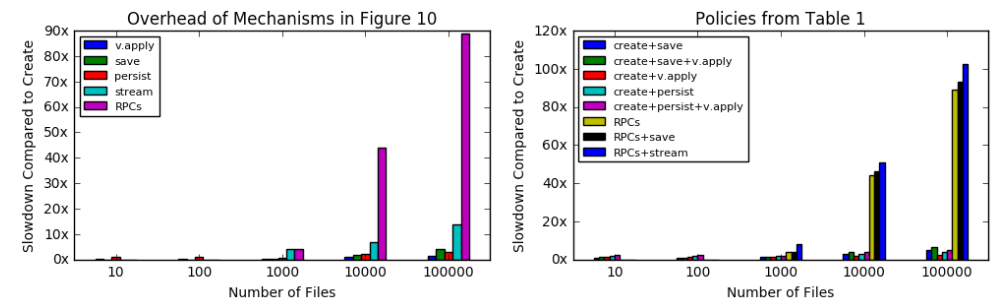
\includegraphics[width=180mm]{figures/results-microbenchmark.png}
\caption{Here's a graph.}
\end{figure*}

\begin{figure}[tb]
\centering
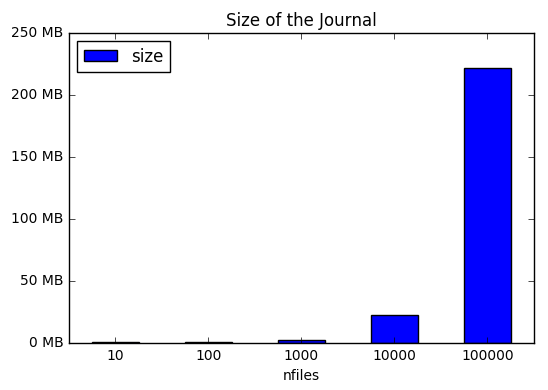
\includegraphics[width=90mm]{figures/results-files.png}
\caption{Here's a graph.}
\end{figure}


\subsubsection{Per phase latencies}
\begin{figure}[tb]
\centering
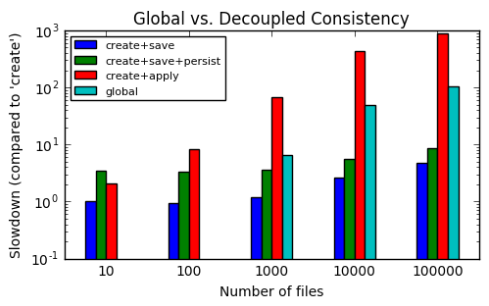
\includegraphics[width=90mm]{figures/global-v-decoupled.png}
\caption{Compared to the \texttt{create} phase, saving and persisting
updates (\texttt{create+save} and \texttt{create+save+persist}) experience only
a 4.79\(\times\) and 8.66\(\times\) slowdown, in the worst case for 100K files.
In contrast, maintaining \texttt{global} consistency is 905.70\(\times\)
slower.  The disadvantage of decoupling the namespace is the merge phase where
updates are applied to the metadata store (\texttt{create+apply}, resulting in a
905.70\(\times\) slowdown for 100K files.}\label{fig:global-v-decoupled}
\end{figure}

%\section{notes}
%Linking clients into our custom libcephfs
%
%Use namespace's recursive data structure to put policies on subtrees
%- consistency: eventual vs. strong, global vs. local
%  - e.g., BatchFS/DeltaFS: eventual, local
%  - e.g., POSIX: strong, global
%  - e.g., PLFS: no consistency
%- fault tolerance: global vs. local
%  - e.g., CephFS: global
%  - e.g., BatchFS/DeltaFS: local
%
%Experimental Setup
%- Ceph: 9 OSDs, 1 MDS, 2 kernel client
%- Workload limitations: blah
%
%Workload: creates
%
%Baseline: 200K creates in the same directory
%- throughput: degrades at 950s
%- CPU utilization: more at 950s
%- inode cache: eviction dominate
%- inodes +- to cache: eviction dominate
%- per-disk throughput: RADOS not bottleneck
%
%Experiment 1: Interference
%
%\subsection{Baseline}
%Experiment 0: creates in the same directory
%- setup: why we use caching, we use the kernel client, how we circumvent max fragment size
%
%Experiment 0: creates with a stat
%- Hypothesis: metadata read pauses creates and requires a snapshot in time
%  - what is more of an overhead: pausing creates and getting a consistent view OR sucking up resources as it reads from RADOS?
%- can we delay snapshot?
%
%Experiment 1: creates with a readdir
%- Hypothesis: shows the cost of synchronization because on a write, the first client drops his caps
%- client0: create 100k, client1: stat at 2 mins
%
%Experiment 2: scale the number of files
%- See if the open/close spike occurs 
%- Try to see why open/close spike is allowed to happen
%- Try to disable all caching -- metadata writes don't ever re-use the inode -- we never ask for it again!
%- client0: create 100k, client1: touch at 2 mins
%
%Experiment 3: see how fast the cache satisfies a read
%- client0: create 100k, stat inodes
%- client0: create 100k, client1: stat inodes
%
%lient 0: creates, client 1 create(s)

\subsection{Journaling Overhead}

Journal to RADOS
Turn off journaling (large segment)
Journal to in-memory OSD 

\subsection{Macrobenchmarks}
updatedb: http://lists.ceph.com/pipermail/ceph-users-ceph.com/2015-July/002768.html




\bibliographystyle{ACM-Reference-Format}
\bibliography{sigproc} 

\end{document}
